% === Revtex Declaration ===
\documentclass[aps, 10pt, english, twoside, pra, nofootinbib, tightenlines, longbibliography]{revtex4-1}

% === All of the Packages I use frequently ===
\usepackage{../../packages/document_config}
\usepackage{../../packages/shared}
\usepackage{../../packages/misc_commands}
\usepackage{subcaption}
\usepackage{enumitem}

\renewcommand{\Events}[1]{\mathcal{S}\br{#1}}
\renewcommand{\tcdot}{\cdot}

% === Causal structure formatting for tikz ===
% =========================
% Causal Structure Diagrams
% =========================
\definecolor{obs_outline}{RGB}{51,157,215}
\definecolor{obs_fill}{RGB}{222,253,255}
\definecolor{obs_text}{RGB}{0,0,0}
\definecolor{lat_outline}{RGB}{251,141,54}
\definecolor{cause}{RGB}{30, 0, 30}
\definecolor{lat_fill}{RGB}{255,213,153}
\definecolor{lat_text}{RGB}{0,0,0}
\tikzset{square/.style={regular polygon,regular polygon sides=4}}
\tikzset{triangle/.style={regular polygon,regular polygon sides=3}}
\tikzset{observed/.style={obs_text, align=center, triangle, thick, draw=obs_outline, fill=obs_fill, inner sep=-0.2em, text width=1.5em}}
\tikzset{latent/.style={lat_text, align=center, circle, thick, draw=lat_outline, fill=lat_fill, text width=1.5em, inner sep=0.2em}}
\tikzset{fade/.style={opacity=0.2}}
\tikzset{unfade/.style={opacity=1.0}}
% TikZ stile to apply keys only on specific beamer overlays
% onslide=<overlay spec>{key=value, key=value, ...}
\tikzset{onslide/.code args={<#1>#2}{%
  \only<#1>{\pgfkeysalso{#2}}%
}}
\providecommand{\p}[1]{#1}
% \tikzset{cause/.style={mid arrow/.style={postaction={decorate,decoration={markings, mark=at position .5 with {\arrow[#1]{stealth}}}}},}}
\tikzset{
    % style to apply some styles to each segment of a path
    on each segment/.style={
        decorate,
        decoration={
            show path construction,
            moveto code={},
            lineto code={
                \path [#1]
                (\tikzinputsegmentfirst) -- (\tikzinputsegmentlast);
            },
            curveto code={
                \path [#1] (\tikzinputsegmentfirst)
                .. controls
                (\tikzinputsegmentsupporta) and (\tikzinputsegmentsupportb)
                ..
                (\tikzinputsegmentlast);
            },
            closepath code={
                \path [#1]
                (\tikzinputsegmentfirst) -- (\tikzinputsegmentlast);
            },
        },
    },
    % style to add an arrow in the middle of a path
    mid arrow/.style={postaction={decorate,decoration={
                markings,
                mark=at position .6 with {\arrow[scale=1.5, cause]{stealth}}
            }}},
}
% =========================
% =========================

\begin{document}
    \title{Causal Compatibility Inequalities Admitting of Quantum Violations in the Triangle Scenario}
    \author{Thomas C. Fraser}
    \email{tcfraser@tcfraser.com}
    \affiliation{Perimeter Institute for Theoretical Physics, Waterloo, Ontario, Canada \\ University of Waterloo, Waterloo, Ontario, Canada}
    % \author{Elie Wolfe}
    % \email{ewolfe@perimeter@institute.ca}
    % \affiliation{Perimeter Institute for Theoretical Physics, Waterloo, Ontario, Canada}
    \date{\today}
    \begin{abstract}
        Quantum correlations are often incompatible with a classical assumption of causal structure. This non-classicality is often known as quantum non-locality, and it is witnessed through the violation of causal compatibility inequalities, such as Bell inequalities. Such inequalities were recently derived for the triangle scenario [arXiv:1609.00672], begging the question: can these inequalities be violated by quantum correlations? Here we answer this affirmatively, and discuss specific triangle scenario inequalities and quantum configurations which manifest non-classical correlations. Numerical optimizations reveal quantum resources potentially qualitatively different from those known previously.
    \end{abstract}
    \maketitle
    \tableofcontents
    \clearpage

    \section{Introduction}
    \label{sec:introduction}
    In recent decades, the technical utility of quantum mechanics has become abundantly clear; quantum computational algorithms such as Shor's algorithm~\cite{Shor_1997} and numerous others~\cite{Jordan_2016} maintain advantage over their classical counterparts. Additionally, classical communications technologies stand to benefit from the nature of quantum mechanics --- a popular example being Quantum Key Distribution~\cite{Bennett_2014}. Any time classical resources are unable to emulate quantum mechanics, there represents an opportunity to exploit the non-classical features of quantum mechanics in order to solve a variety of computational and communicational problems~\cite{Neilsen_Chaung_2011}. Albeit, not all tasks stand to benefit from quantum resources~\cite{Almeida_2010}. Presently, discovering situations or tasks where quantum mechanics offers an advantage, and proving that advantage is genuine, is a primal objective of theoretical quantum information theory. \\

    From a foundational prospective, the majority of attempts to characterize precisely where quantum mechanics and classical mechanics differ have involved Bell inequalities~\cite{Bell_1964}. Originally, Bell inequalities were derived in response to the famous EPR paradox~\cite{EPR_Orig} to rule out hidden variable theories for quantum mechanics. Studying and discovering Bell-type inequalities is useful because a complete set of Bell inequalities provides a systematic way of classifying the \textit{classicality} of a given observation. These inequalities are best understood from the perspective of \term{causal inference} --- a problem which aims to determine which observations can or can not be explained by a hypothesized causal structure. The abstract nature of causal inference is responsible for its presence in numerous scientific fields including machine learning and biology~\cite{Pearl_2009,Pearl_2009_tr}. Inequalities such as Bell inequalities constrain the space of observations that are compatible with a hypothesized causal structure. In the case of the original Bell inequalities, the classical causal model in question is known as the Bell scenario~\cite{Wood_2012} and is depicted in \cref{fig:bell_scenario}. The Bell scenario involves two parties ($A, B$) who each make measurements decided by random settings ($S_A, S_B$) on a shared hidden resource $\la$. Quantum non-classicality in the Bell scenario and related structures have been studied thoroughly since Bell's original work~\cite{Brunner_2013}. However, novel scenarios such as the correlation scenarios proposed by Fritz~\cite{Fritz_2012,Fritz_2014} are arguably less understood compared to the Bell scenario. Here we investigate one particular causal scenario: the triangle scenario (\cref{fig:triangle_scenario}). \\

    The triangle scenario (\cref{fig:triangle_scenario}) is a causal structure composed of $3$ parties labeled $A, B, C$ arranged in a triangular configuration while pair-wise sharing hidden/latent variables $X, Y, Z$. It has been studied extensively in literature before (see~\cite[Fig. 1]{Steudel_2010},~\cite[Fig. 6]{Chaves_2014},~\cite[Fig. 8]{Branciard_2012},~\cite[Fig. 8, Appendix E]{Henson_2014},~\cite[Fig. 3]{Fritz_2012},~\cite[Fig. 1]{Inflation}, $\ldots$). A healthy portion of which the existing literature will be discussed in \cref{sec:triangle_scenario}. For instance \citet{Branciard_2012} noted that characterizing locality in the triangle scenario remained an \textit{open problem} and that identifying causal compatibility inequalities for this configuration \textit{seemed challenging}. The subject of this document is to expound on the developments made towards understanding quantum non-classicality in the triangle scenario. \\

    As a preliminary summary, causal compatibility inequalities were derived for the triangle scenario that are able to be violated by specific quantum-accessible distributions. This was accomplished by combining two previous works. The first, an insight made by \citet{Fritz_2012} regarding the ability to re-interpret the Bell scenario as a portion of the triangle scenario. The second, a new framework for solving causal inference problems developed by Wolfe \emph{et al.}~\cite{Inflation} called \term{The Inflation Technique}. Ultimately, this work serves as a strong indication that the Inflation Technique offers new insights into specifically quantum non-classicality. Moreover, these new inequalities offer an avenue for finding and identifying new forms of non-classicality unknown previously. This report discusses attempts to find such resources with partial success and outlines refinements that can be made for future exploration.\\

    The following paper is organized into the following sections: \Cref{sec:causal_compatibility} recalls important notions from causal inference theory and sets up the notation to be used. \Cref{sec:triangle_scenario} discusses the triangle scenario and its existing research in detail; identifying its stark differences from the Bell scenario and motivates why the triangle scenario was chosen as a case study. \Cref{sec:fritz_distribution} defines and discusses a singular quantum correlation first discovered by \citet{Fritz_2012} which we term the \term{Fritz distribution}. The Fritz distribution was proven to be non-classical without the use of inequalities --- this report derives inequalities that do. \Cref{sec:inflation_technique} briefly summaries the Inflation Technique in the context of this work. Although the summary presented here is sufficient, the original work~\cite{Inflation} offers a more concrete and pedagogical introduction. \Cref{sec:deriving_inequalities} demonstrates how the inflation technique can be used to derive causal compatibility inequalities for the triangle scenario that are violated by quantum-accessible distributions. A sample of these inequalities are presented at the end of \cref{sec:deriving_inequalities} as well as \cref{sec:web_inequality,sec:symmetic_web_inequality}. Finally, \cref{sec:violations_noise} mentions a method for parameterizing the space of quantum-accessible distributions which is used to numerically optimize against our derived inequalities in search of stronger types of non-classicality. Additionally, the Fritz distribution is subjected to noise in order to measure the robustness of the derived inequalities.

    \section{Causal Compatibility}
    \label{sec:causal_compatibility}
    The task of causal inference aims to determine whether or not a given family of observed probability distributions can be explained by a proposed causal mechanism~\cite{Pearl_2009}. If a set of observed distributions can be explained by the hypothesized causal mechanism, then the observations are said to be \textit{compatible} with the causal mechanism. In order to define compatibility rigorously, we first need to formally define what is meant by ``set of observations''.

    \subsection{Marginal Models}
    Given a set of observable variables $\jointvar = \bc{v_1, \ldots, v_k}$ where each $v \in \jointvar$ is a statistical random variable, one can conceivably make a measurement over of these variables and obtain a joint probability distribution $\prob[\jointvar] = \prob[v_1,\ldots,v_n]$. More generally however, and depending on the context, it is possible to make a measurement on a portion of the system $V \subset \jointvar$ in order to obtain a marginal distribution $\prob[V]$. With complete generality however, one could in principle make a measurement on a collection of portions of the system $\mscenario = \bc{V_1, \ldots, V_m \mid \forall i : V_i \subseteq \jointvar}$ obtaining a collection of marginal probability distributions $\bc{\prob[V_1], \ldots, \prob[V_m] \mid \forall i: V_i \in \mscenario}$. \\

    The set $\mscenario = \bc{V \mid V \subseteq \jointvar}$ of subsets of $\jointvar$ is referred to as the \term{marginal scenario} and each element $V \in \mscenario$ is termed a \term{(marginal) context} of $\mscenario$. The complete set of marginal distributions is referred to as the \term{marginal model} and is denoted with an superscript $\prob^{\mscenario}$:
    \[ \prob^{\mscenario} = \bc{\prob[V] \mid V \in \mscenario} \]
    A marginal model acts as the most general description of a family of observations that can be made over $\jointvar$. Strictly speaking, as defined by~\cite{Fritz_2011}, a marginal scenario forms an \textit{abstract simplicial complex} where it is required that all subsets of contexts are also contexts.
    \[ \forall V \in \mscenario, V' \subset V : V' \in \mscenario \]
    Throughout this document, we only consider (without loss of generality) the \textit{maximal} marginal scenario; restricting our focus to the largest contexts in the marginal scenario. Additionally, all marginal scenarios are taken to be \text{complete} in the sense that the marginal scenario covers the complete set of observable variables $\jointvar$.
    \[ \jointvar = \bigcup_{V \in \mscenario} V \]

    \subsection{Causal Structure}
    A \term{causal structure} abstractly represents the hypothesized causal mechanism. Mathematically, a causal structure is a directed acyclic graph $\graph = \br{\nodes, \edges}$ of nodes $\nodes$ and edges $\edges$ as defined in \cref{sec:graph_theory}. The nodes of a causal structure are random variables and are classified into two disjoint classes: the \term{latent nodes} $\nodes_L$ representing the set of nodes that are unobservable and the \term{observed nodes} $\nodes_O$. The latent nodes of a causal structure represent completely hidden variables that are hidden by some fundamental process or cannot be measured due to other limitations. The observed nodes represent random variables that are measurable and in practice will be observed by the marginal model $\prob^\mscenario$. The edges $\edges$ of a causal structure represent casual influence between variables within the causal structure. \\

    A number of causal structures are depicted throughout this document (see \cref{fig:bell_scenario,fig:triangle_scenario} as well as \cref{fig:inflations}). As an example, the triangle scenario has $3$ observable nodes and $3$ latent nodes,
    \[ \nodes_{O} = \bc{A, B, C} \qquad \nodes_{L} = \bc{X, Y, Z} \]
    along with $6$ edges indicating that the latent nodes $\bc{X, Y, Z}$ cause and influence the observed nodes $\bc{A, B, C}$.
    \[ \edges = \bc{\bc{X \to A}, \bc{Y \to A}, \bc{Y \to B}, \bc{Z \to B}, \bc{Z \to C}, \bc{X \to C}} \]

    \subsection{Compatibility}
    \label{sec:compatibility}

    Now that the notions of a causal structure $\graph$ and a marginal model $\prob^{\mscenario}$ are defined, it is now possible to precisely define the notion of compatibility between the two. Intuitively, the causal connections within $\graph$ should restrict and limit the set of possible observations that can be made on $\graph$. Namely, if each variable $n \in \nodes$ is caused by its parents $\Pa[\graph]{n}$, then $n$ should be independent of all other variables that are not its descendants. This is known as the \term{local Markov property}:
    \[ n \indep \nodes \setminus \De[\graph]{n} \mid \Pa[\graph]{n} \quad \forall n \in \nodes \eq \label{eq:local_markov_property} \]
    Where $\indep$ denotes statistical independence. With this as motivation, we define a set of \term{causal parameters} for a causal structure $\graph$ to be a specification of a conditional distribution for every variable $n \in \nodes$ given its parents:
    \[ \bc{\prob[n \mid \Pa[\graph]{n}] \mid n \in \nodes} \eq \label{eq:causal_parameters} \]
    It is important to note that a set of causal parameters is not unique; the numerical nature of set of causal parameters is a \text{choice}. Altogether, a marginal model $\prob^{\mscenario}$ is \term{compatible} with a causal structure $\graph$ if there exists a choice of causal parameters such that each context $\prob[V] \in \prob^{\mscenario}$ can be \textit{recovered} from the following series of operations:
    \begin{enumerate}
        \item Obtain a joint probability distribution over \textit{all} variables of the causal structure using the chosen casual parameters:\footnote{Here $\prod$ denotes the product distribution $\prod_{n \in \nodes} \prob[n \mid \Pa[\graph]{n}] = \prob[n_1 \mid \Pa[\graph]{n_1}] \times \cdots \times \prob[n_k \mid \Pa[\graph]{n_k}]$.}
        \[ \prob[\nodes] = \prod_{n \in \nodes} \prob[n \mid \Pa[\graph]{n}] \eq \label{eq:local_markov_property_operation}\]
        This step ensures that the local Markov property (\cref{eq:causal_parameters}) holds for all variables $n \in \nodes$.
        \item Marginalize over the latent variables of $\graph$ to obtain a joint distribution over the observed variables $\nodes_O$:
        \[ \prob[\nodes_O] = \sum_{\nodes_L} \prob[\nodes] \eq \label{eq:observable_marginalization} \]
        \item Finally marginalize over the observed nodes not in $V$ to obtain $\prob[V]$:
        \[ \prob[V] = \sum_{\nodes_O \setminus V} \prob[\nodes_O] \eq \label{eq:context_marginalization} \]
    \end{enumerate}
    It is important to note that compatibility between $\prob^{\mscenario}$ and $\graph$ requires that it is possible to recover \textit{each} context $\prob[V] \in \prob^{\mscenario}$ from the \textit{same} set of causal parameters. If it is not possible for $\prob^{\mscenario}$ to be recovered for \textit{any} choice of causal parameters, then $\prob^{\mscenario}$ is \term{incompatible}.

    \subsection{Inequalities}
    As defined in \cref{sec:compatibility}, determining compatibility is equivalent to determining if a set of causal parameters exists with the above-mentioned properties. In practice however, checking causal parameters systemically is intractable, especially when the cardinality (number of outcomes) of the latent variables is unspecified. Instead, \term{causal compatibility inequalities}\footnote{We refer to these inequalities as ``causal compatibility inequalities'' instead of simply Bell inequalities for two reasons. First, ``Bell inequalities'' usually are associated specifically with the Bell scenario/Bell causal structure. Second, the inequalities derived in this work are fundamentally distinct from a typical Bell inequality in that these inequalities are \textit{polynomial} over $\prob^{\mscenario}$ instead of \textit{linear}.} are probabilistic inequalities defined over the marginal contexts $\prob[V] \in \prob^{\mscenario}$ within the marginal model. If a marginal model $\prob^{\mscenario}$ happens to \textit{violate} any causal compatibility inequality, then that marginal model is definitely \textit{incompatible}. In \cref{sec:deriving_inequalities}, a brief discussion of existing techniques for deriving these inequalities will take place.\\

    Unfortunately, a singular inequality can not prove that a given marginal model is \textit{compatible}, only \textit{incompatible}. Instead, a \textit{complete characterization} of compatibility would consist of a complete set of all valid causal compatibility inequalities; satisfaction of a complete set of inequalities does prove compatibility. Currently however, it is unknown how to obtain a complete characterization for any given causal structure, including the triangle scenario.  \\

    From the perspective of identifying quantum non-classicality, the causal structure $\graph$ acts as the classical hypothesis for a particular marginal model $\prob^{\mscenario}$. Therefore, non-classicality becomes synonymous with incompatibility: if a marginal model $\prob^{\mscenario}$ is incompatible, then it is non-classical. Henceforth, we will use these two terms interchangeably. From a resource standpoint, if the non-classicality of $\prob^{\mscenario}$ can be witnessed by an inequality $I$, but $\prob^{\mscenario}$ can be implemented using quantum states and measurements, then the causal compatibility inequality $I$ represents a concrete task where quantum resources out-perform classical resources.

    \section{Triangle Scenario}
    \label{sec:triangle_scenario}

    \begin{figure}
    \begin{center}
        \begin{minipage}[t]{.48\textwidth}
            \centering
            \scalebox{1.0}{\begin{tikzpicture}[scale=1]
    \begin{scope}[every node/.style=observed]
        \node (B) at (2, 2) {$\p{B}$};
        \node (A) at (-2, 2) {$\p{A}$};
        \node (Z) at (2, 0) {$S_{\p{B}}$};
        \node (X) at (-2, 0) {$S_{\p{A}}$};
    \end{scope}
    \begin{scope}[every node/.style=latent]
        \node (Y) at (0, 0.5) {$\la$};
    \end{scope}
    \begin{scope}[every path/.style={draw=cause, thick}]
        \path[postaction={on each segment={mid arrow}}]
        (X) -- (A)
        (Y) -- (A)
        (Y) -- (B)
        (Z) -- (B);
    \end{scope}
\end{tikzpicture}}
            \caption{The Bell scenario consisting of two observers $\p{A}, \p{B}$ together with measurement settings $S_{\p{A}}$ and $S_{\p{B}}$ respectively. The shared hidden variable is labeled $\la$.}
            \label{fig:bell_scenario}
        \end{minipage}\hspace{0.04\textwidth}%
        \begin{minipage}[t]{.48\textwidth}
            \centering
            \scalebox{1.0}{\begin{tikzpicture}[scale=1]
    \begin{scope}[every node/.style=observed]
        \node (C) at (-2, 0) {$C$};
        \node (B) at (2, 0) {$B$};
        \node (A) at (0, {2*sqrt(3)}) {$A$};
    \end{scope}
    \begin{scope}[every node/.style=latent]
        \node (X) at (-1, {sqrt(3)}) {$X$};
        \node (Y) at (1, {sqrt(3)}) {$Y$};
        \node (Z) at (0, 0) {$Z$};
    \end{scope}
    \begin{scope}[every path/.style={draw=cause, thick}]
        \path[postaction={on each segment={mid arrow}}]
        (X) -- (A)
        (X) -- (C)
        (Y) -- (A)
        (Y) -- (B)
        (Z) -- (B)
        (Z) -- (C);
    \end{scope}
\end{tikzpicture}}
            \caption{The casual structure of the triangle scenario. Three variables $A,B,C$ are observable, while $X, Y, Z$ are latent variables.}
            \label{fig:triangle_scenario}
        \end{minipage}
    \end{center}
    \end{figure}
    Discovering quantum non-classicality in any causal structure is desirable, so why, in particular, is it important to do so in the triangle scenario? As was mentioned in \cref{sec:introduction,sec:causal_compatibility}, the \term{triangle scenario} (\cref{fig:triangle_scenario}) is a causal structure $\graph$ consisting of $3$ observable variables $A, B, C$ arranged in a triangular configuration while pair-wise sharing latent variables $X, Y, Z$. \\

    Following the definition of causal compatibility from \cref{sec:causal_compatibility}, a distribution $\prob[\nodes_{O}] = \prob[ABC]$ is compatible with the triangle scenario if and only if there exists a choice of causal parameters $\bc{\prob[A|X,Y],\prob[B|Y,Z],\prob[C|Z,X],\prob[X],\prob[Y],\prob[Z]}$ such that the joint distribution $\prob[\nodes] = \prob[ABCXYZ]$ is a product over the causal parameters,
    \[ \prob[ABCXYZ] = \prob[A|X,Y]\prob[B|Y,Z]\prob[C|Z,X]\prob[X]\prob[Y]\prob[Z] \]
    And also, the given distribution $\prob[ABC]$ is a marginalization of $\prob[ABCXYZ]$ over $X, Y, Z$:
    \[ \prob[ABC] = \sum_{X,Y,Z}\prob[A|X,Y]\prob[B|Y,Z]\prob[C|Z,X]\prob[X]\prob[Y]\prob[Z] \eq \label{eq:triangle_compatibility} \]

    For certain causal structures, the conditional independence relations provided by $d$-separation relations are a sufficient characterization of compatibility. Recently, \citet{Henson_2014}, classified the triangle scenario as an \textit{interesting} causal structure in the sense that conditional independence relations \textit{do not} provide a sufficient characterization of non-classicality.\footnote{Note that the triangle scenario possesses \textit{zero} conditional independence relations over the observable nodes $A, B, C$.} Moreover, \citet{Inflation} concretely demonstrate that the space classical distributions on the triangle scenario is non-convex, unlike the Bell scenario. It can be argued that convexity of the Bell scenario distributions is partially responsible for the wealth of knowledge that is known about the Bell scenario. It is also reasonable to speculate that quantum non-classicality in the triangle can be translated directly into a computational advantage for certain computational circuits~\cite{Terhal_2002}. Characterizing quantum non-classicality for interesting causal structures remains an unsolved problem, and the triangle scenario is a small, non-trivial case study. \\

    Additionally, \citet{Fritz_2012} demonstrated that the triangle scenario is the \textit{smallest} correlation scenario\footnote{Correlation scenarios differ from the Bell scenario in that measure setting variables are non-existence in correlation scenarios.} in which their exists incompatible, quantum distributions by explicitly mentioning one which we have elected to call the Fritz distribution (see \cref{sec:fritz_distribution}). Fritz's proof of non-classicality does not involve compatibility inequalities, but instead mentions that inequalities would be helpful for characterizing non-classical in the triangle scenario. \\

    Finally \citet{Inflation} proposed the Inflation Technique (summarized in \cref{sec:inflation_technique}), a novel tool for solving causal inference problems. Using the inflation technique, they were able to prove incompatibility between the triangle scenario and the $W$-type distribution; a quantum non-accessible distribution whose incompatibility is not witness-able by \textit{any} entropic inequalities or any other known constraints. Therefore as a an algorithmic framework, the Inflation Technique comes closer to characterizing non-classicality in the triangle scenario that all others. \\

    It is worth noting that a number of causal compatibility inequalities for the triangle scenario have been derived in previous works. For example, \citet{Steudel_2010} derived an inequality for a series of causal structures with $n \in \N$ variables where at most $c \in \N$ share a common ancestor. The triangle scenario is a special case with $c = 2$, $n = 3$. Moreover, \citet{Henson_2014} derive a family of entropic inequalities constraining the set of compatible correlations. Most impressively, \citet{Inflation} derive a family of polynomial, $2$-outcome, causal compatibility inequalities; $37$ non-trivial representatives are printed in~\cite{Inflation}. \\

    As a preliminary search for quantum incompatibility in the triangle scenario, we performed numerical optimizations using bipartite qubit density matrices and $2$-outcome POVM measurements against the compatibility inequalities printed in~\cite{Inflation} as well as the entropic inequalities presented by \citet{Henson_2014}. Unfortunately, none of these inequalities could be violated. These early results suggest, although do not prove, that quantum non-classical does not exist in the triangle scenario for \textit{two-outcome} measurements. We make \textit{no claim} that this is a universal truth and simply take it as motivation to explore incompatibility in triangle scenario for a degree of outcomes. \\


    In conclusion, the triangle scenario is a causal structure whose non-classicality remains an open problem. The triangle scenario is a desirable case study because there is a quantum distribution that is known to be incompatible, but no previously known inequalities were able to witness its incompatibility. This failure represents a gap in our understanding of quantum non-classicality, where recent developments (namely the Inflation Technique) have made partial progress. This document expands on our understanding of non-classicality in the triangle scenario and also our understanding on how to find inequalities using the Inflation Technique for interesting causal structures in general.

    \section{Fritz Distribution}
    \label{sec:fritz_distribution}
    \begin{figure}
    \begin{center}
        \scalebox{1.0}{\begin{tikzpicture}[scale=1]
    \begin{scope}[every node/.style=observed]
        \node (C) at (0, -2.5) {$C$};
        \node (B) at (2, 2) {$B$};
        \node (A) at (-2, 2) {$A$};
    \end{scope}
    \begin{scope}[every node/.style=latent]
        \node (X) at (-2, 0) {$S_A$};
        \node (Y) at (0, 0.5) {$\la$};
        \node (Z) at (2, 0) {$S_B$};
    \end{scope}
    \begin{scope}[every path/.style={draw=cause, thick}]
        \path[postaction={on each segment={mid arrow}}]
        (X) -- (A)
        (X) -- (C)
        (Y) -- (A)
        (Y) -- (B)
        (Z) -- (B)
        (Z) -- (C);
    \end{scope}
\end{tikzpicture}}
        \caption{The triangle scenario re-imagined to mimic the Bell scenario. The measurement settings $S_{\p{A}},S_{\p{B}}$ are latent nodes unlike the Bell scenario (\cref{fig:bell_scenario}).}
        \label{fig:triangle_scenario_with_fritz_bell_embedded}
    \end{center}
    \end{figure}

    As was originally noticed by \citet{Fritz_2012}, it is possible to construct quantum distributions incompatible with the triangle scenario by utilizing quantum distributions incompatible with the familiar Bell scenario. To explain, imagine rearranging the triangle into the configuration depicted in \cref{fig:triangle_scenario_with_fritz_bell_embedded} and contrast it with the Bell scenario of \cref{fig:bell_scenario}. Evidently, under the correct relabeling, large portions of the Triangle Scenario resemble the Bell Scenario. The crucial distinction is that the measurement settings $S_{\p{A}}, S_{\p{B}}$ are \textit{observable variables} in the Bell scenario but become \textit{latent variables} in the triangle scenario. In order to embed distributions that are incompatible with the Bell scenario into the triangle scenario, the latent nodes $S_{\p{A}}, S_{\p{B}}$ need to be observable and independent of the shared latent node $\la$. This can be accomplished by having $C$ ``measure'' the measurement settings $S_{\p{A}}, S_{\p{B}}$ and announce them as an outcome. Consequently, any distribution over $\p{A}, \p{B}, S_{\p{A}}, S_{\p{B}}$ that is incompatible with Bell scenario is also incompatible with the triangle scenario provided that $C$ is \textit{perfectly correlated} with $S_{\p{A}}, S_{\p{B}}$. Understandably there are numerous ways that this can be accomplished, albeit we will focus on elucidating an exemplary method. \\

    The \term{Fritz distribution}, denoted $\prob[\fritz]$, is a quantum-accessible distribution known to be incompatible with the triangle scenario~\cite{Fritz_2012}. In the Fritz distribution, each of the variables $A,B,C$ have $4$ possible outcomes. Explicitly, $\prob[\fritz]$ can be written as:
    \begin{align*}
    \eq \label{eq:fritz_dist}
    \begin{split}
        \prob[\fritz][000] = \prob[\fritz][110] = \prob[\fritz][021] = \prob[\fritz][131] = \prob[\fritz][202] = \prob[\fritz][312] = \prob[\fritz][233] = \prob[\fritz][323] &= \f{1}{32}\br{2 + \sqrt{2}} \\
        \prob[\fritz][010] = \prob[\fritz][100] = \prob[\fritz][031] = \prob[\fritz][121] = \prob[\fritz][212] = \prob[\fritz][302] = \prob[\fritz][223] = \prob[\fritz][333] &= \f{1}{32}\br{2 - \sqrt{2}}
    \end{split}
    \end{align*}
    Here the notation $\prob[\fritz][abc] = \prob[\p{ABC}][abc] = \prob[][\p A=a,\p B=b,\p C=c]$ is used as shorthand. The Fritz distribution is best visualized as a $4 \times 4 \times 4$ grid of possible outcomes as depicted in \cref{fig:fritz_distribution_visualized}. From this diagram, it can be seen that each of $\p{C}$'s outcomes restricts the possible outcomes for $\p A,\p B$ into a $2 \times 2$ block. If one writes the outcome labels $\bc{0,1,2,3}$ in binary $\bc{00,01,10,11}$, it can be seen that the left-hand bits for $\p A$ and $\p B$ (respectively denoted $\p A_l$, $\p B_l$) are fixed by the outcome of $\p C$. Pursuant to the embedding of~\cref{fig:triangle_scenario_with_fritz_bell_embedded} the left-hand bits emulate the measurement settings $S_{\p A}$ and $S_{\p B}$ and the right-hand bits emulate a two-outcome measurement performed by $A, B$ as they would in~\cref{fig:bell_scenario}. Specifically, $\p C$'s bits are perfectly correlated with the left-bits of $A,B$; $\p C_l = \p A_l$ and $\p C_r = \p B_l$.
    \begin{figure}
    \begin{center}
            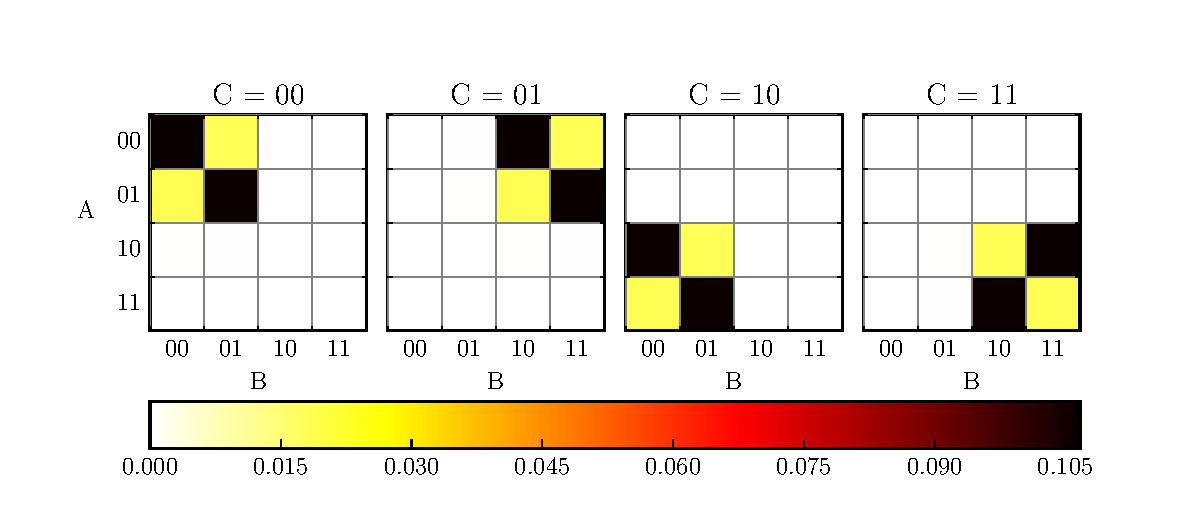
\includegraphics[scale=0.6]{../../figures/distributions/fritz_dist_plotted_bits.pdf}
            \vspace{-0.2in}
            \[ \probplotvalue{253, 253, 84} = \f{1}{32}\br{2 - \sqrt{2}} \qquad \probplotvalue{11, 1, 0} = \f{1}{32}\br{2 + \sqrt{2}}\]
            \caption{The Fritz distribution visualized using a $4 \times 4 \times 4$ grid. The $4$ outcomes of $A,B,C$ are written in binary as a doublet of bits to illustrate that certain bits act as measurement pseudo-settings.}
            \label{fig:fritz_distribution_visualized}
    \end{center}
    \end{figure}
    Consequently, it is possible to define the correlation between the right-hand bits of $A$ and $B$ as the probability that $A_r$ and $B_r$ are equal less the probability that they differ:
    \[ \ba{\p A_r \p B_r} = \prob[\p A_r \p B_r][00] + \prob[\p A_r \p B_r][11] - \prob[\p A_r \p B_r][01] - \prob[\p A_r \p B_r][10] \]
    Provided that $C$ is perfectly correlated with $A_l$ and $B_l$, any Bell inequality for the Bell scenario defined over $\p{A}, \p{B}, S_{\p{A}}, S_{\p{B}}$ can be directly converted to an inequality for the triangle scenario using the following mapping:
    \[ \p{A}, \p{B}, S_{\p{A}}, S_{\p{B}} \mapsto \p{A_r}, \p{B_r}, \p A_l, \p B_l \]
    As an example, the famous CHSH inequality~\cite{CHSH_Original},
    \[ \ba{\p A\p B | S_{\p{A}} = 0, S_{\p{B}} = 0} + \ba{\p A\p B | S_{\p{A}} = 0, S_{\p{B}} = 1} + \ba{\p A\p B | S_{\p{A}} = 1, S_{\p{B}} = 0} - \ba{\p A\p B | S_{\p{A}} = 1, S_{\p{B}} = 1} \leq 2 \]
    Can be written for the right-bits of $A$ and $B$,
    \[ \ba{\p A_r \p B_r|\p C = 00} + \ba{\p A_r \p B_r|\p C = 01} + \ba{\p A_r \p B_r|\p C = 10} - \ba{\p A_r \p B_r|\p C = 11} \leq 2 \eq \label{eq:CHSH} \]
    Therefore, every compatible distribution $\prob[ABC]$ where $C$ is perfectly correlated $A_l,B_l$ must satisfy \cref{eq:CHSH}. Substituting the Fritz distribution (\cref{eq:fritz_dist}) into \cref{eq:CHSH} yields maximal violation~\cite{Cirelson_1980},
    \[ 3 \br{\f{1}{\sqrt{2}}} - \br{-\f{1}{\sqrt{2}}} = 2\sqrt{2} \not \leq 2 \]
    Therefore, the Fritz distribution is incompatible with the triangle scenario as promised. \\

    The Fritz distribution $\prob[\fritz]$ is of special interest because it can be realized as a set of quantum states and measurements on the quantum causal model depicted in \cref{fig:triangle_scenario_quantum_model}. The shared resource between $A$ and $B$ (graphically denoted $\la$ in \cref{fig:triangle_scenario_with_fritz_bell_embedded}) is the maximally entangled Bell state:
    \[ \ket{\Phi^+} = \f{1}{\sqrt{2}}\br{\ket{00} + \ket{11}} \qquad \rho_{AB} = \ket{\Phi^+}\bra{\Phi^+} \]
    While the states shared with $C$ are the following mixed states:
    \[ \rho_{BC} = \rho_{CA} = \f{\ket{00}\bra{00} + \ket{11}\bra{11}}{2} \]
    The measurements employed by $A,B$ and $C$ are separable, projective measurements,
    \begin{align*}
        M_{A} &= \bc{\ket{0\psi_{1}}\bra{0\psi_{1}}, \ket{0\psi_{5}}\bra{0\psi_{5}}, \ket{1\psi_{3}}\bra{1\psi_{3}}, \ket{1\psi_{7}}\bra{1\psi_{7}}} \\
        M_{B} &= \bc{\ket{\psi_{6}0}\bra{\psi_{6}0}, \ket{\psi_{2}0}\bra{\psi_{2}0}, \ket{\psi_{0}1}\bra{\psi_{0}1}, \ket{\psi_{4}1}\bra{\psi_{4}1}} \\
        M_{C} &= \bc{\ket{00}\bra{00}, \ket{10}\bra{10}, \ket{01}\bra{01}, \ket{11}\bra{11}}
    \end{align*}
    Where $\ket{\psi_n}$ is shorthand for,
    \[ \ket{\psi_n} = \f{1}{\sqrt{2}}\br{\ket{0} + e^{in/4}\ket{1}} \]
    Using the above states and measurements, the Fritz distribution $\prob[\fritz]$ can be recovered using the following:
    \[ \prob[ABC] = \Tr\bs{\netperm^\intercal \rho_{AB}\otimes\rho_{BC}\otimes\rho_{CA} \netperm M_{A}\otimes M_{B} \otimes M_{C}} \]
    Where $\netperm$ is a $64 \times 64$ permutation matrix to be elaborated in \cref{sec:perm_matrix}. \\

    Before continuing it is worth noting that \cref{eq:fritz_dist} is non-unique. Any distribution that is equal to \cref{eq:fritz_dist} via a permutation of outcomes or exchange of parties is should also be referred to as a Fritz distribution. Moreover, the quantum realization presented here is not unique either. Nonetheless for concreteness, \cref{eq:fritz_dist} is taken as \textit{the} Fritz distribution throughout this paper. Moreover, the quantum implementation of the Fritz distribution presented above is non-unique also. For example, it is possible to implement the Fritz distribution using maximally entangled Bell states for each shared resource $\rho_{AB}, \rho_{BC}, \rho_{CA}$ provided there is an appropriate adjustment to the measurements $M_A, M_B, M_C$. Ultimately however, only $\rho_{AB}$ is required to be entangled in order to reproduce the Fritz; after-all, $C$ is simply classically announcing $A_r$ and $B_r$ as he receives them. \\

    Additionally, it is important to understand the domain in which Fritz's proof of incompatibility is valid. Specifically, \cref{eq:CHSH} can only be applied to the triangle scenario where there exists perfect correlation between $\p C$'s outcomes and the measurement pseudo-settings (left-bits) of $\p A$ and $\p B$. The details of this restriction are discussed and proven in Fritz's original work~\cite{Fritz_2012}. As such, the incompatibility proof employed by Fritz is not applicable to any distribution that significantly deviates from the Fritz distribution presented above. For example, if one combines \cref{eq:fritz_dist} with more and more uniform noise, at what point does the resultant distribution transition from incompatibility to compatibility? This problem is discussed more in \cref{sec:noise}. \\

    Upon reflection, the Fritz distribution can rightly be considered slightly manufactured. The phenomenology associated with Bell non-locality or Bell incompatibility are well understood; examining these distributions under a triangle scenario embedding offers no additional perspective onto the types of resources made accessible by quantum mechanics. Therefore, it is desirable to find incompatible quantum distributions that are qualitatively different than those previously considered for the Bell scenario. \citet{Fritz_2012} presented the following problem: \textit{Find an example of non-classical quantum correlations in the triangle scenario together with a proof of its non-classicality which does not hinge on Bell’s Theorem.}\footnote{In the way Fritz defines, \textit{non-classical} correlations are the class of \textit{incompatible} correlations.} The problem is understandably stated ambiguously as it is not yet entirely clear how to distinguish between non-classical distributions on differing causal structures. In order to remove some of the ambiguity, consider the following refinements of the problem:
    \begin{enumerate}[label=\textbf{R.\arabic*}]
        \item \label{r:1} Find proofs for causal incompatibility of quantum distributions on the triangle scenario that are \textit{not} reliant on perfect correlations.
        \item \label{r:2} Find incompatible quantum distributions on the triangle scenario that satisfy all Bell scenario inequalities under Fritz-type embeddings.
        \item \label{r:3} Find incompatible quantum distributions that require entanglement in more than one shared state.
    \end{enumerate}
    The remainder of this document focuses on a positive solution to \ref{r:1} but leaves \ref{r:2} and \ref{r:3} partially unanswered.

    \section{Inflation Technique}
    \label{sec:inflation_technique}
    The \term{Inflation Technique}, invented by \citet{Inflation} and inspired by the \textit{do calculus} and \textit{twin networks} of \citet{Pearl_2009}, is a family of causal inference techniques that can be used to determine if a marginal model $\prob^{\mscenario}$ is compatible or incompatible with a given causal structure $\graph$. As a preliminary summary, the inflation technique begins by \textit{augmenting} a causal structure with additional copies of its nodes, producing an \textit{inflated} causal structure, and then exposes how causal inference tasks on the inflated causal structure can be used to make inferences on the original causal structure. As a example, inflations of the triangle scenario are depicted in \cref{fig:inflations}. Copies of nodes in the inflated causal structure are distinguished by an additional subscript called the \term{copy-index}. For example node $A$ of \cref{fig:triangle_scenario} has copies $A_1, A_2, A_3, A_4$ in the \textit{Web inflation} of \cref{fig:the_web_inflation}. All such copies are deemed equivalent via a \term{copy-index equivalence} relation denoted `$\sim$'. A copy-index is effectively arbitrary, so we will refer to an arbitrary inflated copy of $A$ as $A'$.
    \[ A \sim A_1 \sim A' \not\sim B \sim B_1 \sim B' \]
    We preemptively generalize the notion of copy-index equivalence to other mathematical objects like sets, graphs, and groups by saying that $X \sim Y$ if and only if $X = Y$ upon removal of the copy-index. Equipped with the common graph-theoretic terminology and notation of \cref{def:graph_terms}, an inflation can be formally defined as follows:
    \begin{definition}
        An \term{inflation} of a causal structure $\graph$ is another causal structure $\graph'$ such that:
        \[ \forall n' \in \nodes': \AnSub[\graph']{n'} \sim \AnSub[\graph]{n} \eq \label{eq:inflation_defn}\]
        Verbally, for each inflated node $n'$, the ancestral sub-graph of $n'$ in $\graph'$ is equivalent to its counterpart in $\graph$ up to copy-index.
    \end{definition}
    The motivation behind this definition is that if the ancestry of each node $n'$ in $\graph'$ plays the \textit{exact same} role as the ancestry of its source copy $n$ in $\graph$, then every compatible joint distribution $\prob[\nodes]$ on $\graph$ can be used to \textit{create} compatible joint distributions on $\graph'$. \\

    To do this, first notice that every compatible joint distribution $\prob[\nodes]$ uniquely defines a set of causal parameters for $\graph$. It is possible to obtain these causal parameters by computing the single-variable marginal distributions of $\prob[\nodes]$,
    \[ \forall n \in \nodes : \prob[n\mid \Pa[\graph]{n}] = \sum_{\nodes \setminus n} \prob[\nodes] \eq \label{eq:unique_causal_parameters}\]
    Now it is possible to make use of the inflation criteria (\cref{eq:inflation_defn}) which at least enforces that $\Pa[\graph']{n'} \sim \Pa[\graph]{n}$. From this, one can create a set of \term{inflated causal parameters} using \cref{eq:unique_causal_parameters},
    \[ \forall n' \in \nodes' : \prob[n'\mid \Pa[\graph']{n'}] \defined \prob[n\mid \Pa[\graph]{n}] \eq \label{eq:inflated_causal_parameters} \]
    Which in turn uniquely defines a compatible joint distribution $\prob[\nodes']$ on $\graph'$\footnote{Of course, there exists compatible joint distributions on $\nodes'$ that can not be constructed in this manner. The claim is that all joint distributions that are constructed in this way are compatible.}.
    \[ \prob[\nodes'] = \prod_{n' \in \nodes'} \prob[n'\mid \Pa[\graph']{n'}] \eq \label{eq:unique_causal_parameters_inflated}\]
    Together, \cref{eq:unique_causal_parameters,eq:inflated_causal_parameters,eq:unique_causal_parameters_inflated} form the \term{weak inflation lemma}: compatible joint distributions over $\nodes$ induce compatible joint distributions over $\nodes'$. Before generalizing to the inflation lemma, a careful observation needs to be made. For any pair of subsets of nodes $N \subseteq \nodes$ and $N' \subseteq \nodes'$ that are equivalent up to copy-index $N \sim N'$, if $\AnSub[\graph]{N} \sim \AnSub[\graph']{N'}$ then any compatible \textit{marginal} distribution $\prob[N]$, where $N \subset \nodes$, induces a compatible marginal distribution $\prob[N']$ over $N'$. In fact, $N'$ must contain no duplicate nodes up to copy index and thus $\prob[N] = \prob[N']$. These subsets of nodes are so essential to the Inflation Technique they are assigned a special name: sets $N' \subseteq \nodes'$ as called the \term{injectable sets} of $\graph'$ and $N \subset \nodes$ the \term{images of the injectable sets} of $\graph$.
    \begin{align*}
        \Inj[\graph]{\graph'} &\defined \bc{N' \subseteq \nodes' \mid \exists N \subseteq \nodes : N \sim N'} \\
        \ImInj[\graph]{\graph'} &\defined \bc{N \subseteq \nodes \mid \exists N' \subseteq \nodes' : N \sim N'}
    \end{align*}
    Injectable sets are incredibly useful for causal compatibility because they allow one to extend the weak inflation lemma to \textit{the} inflation lemma:
    \begin{lemma}
        \label[lemma]{lem:inflation}
        \term{The Inflation Lemma}~\cite[Lemma 3]{Inflation} Given a particular inflation $\graph'$ of $\graph$ and a marginal model $\bc{\prob[N] \mid N \in \ImInj[\graph]{\graph'}}$ compatible with $\graph$ then all marginal models $\bc{\prob[N'] \mid N' \in \Inj[\graph]{\graph'}}$ are compatible with $\graph'$ provided that $\prob[N] = \prob[N']$ for all instances where $N \sim N'$.
    \end{lemma}
    Diagrammatically, \cref{lem:inflation} can be visualized as follows:

    \begin{center}
        \begin{tikzpicture}
            \pgfmathsetmacro{\vs}{2.2};
            \pgfmathsetmacro{\hs}{5.2};
            \draw (0*\hs,0*\vs) node[](pn){$\underbrace{\bc{\prob[N] \mid N \in \ImInj[\graph]{\graph'}}}_{\text{compatible with $\graph$}}$};
            \draw (1*\hs,0*\vs) node[](cp){$\bc{\prob[n\mid \Pa[\graph]{n}] \mid n \in \nodes}$};
            \draw (1*\hs,-1*\vs) node[](cp_){$\bc{\prob[n'\mid \Pa[\graph']{n'}] \mid n' \in \nodes'}$};
            \draw (0*\hs,-1*\vs) node[](pn_){$\underbrace{\bc{\prob[N'] \mid N' \in \Inj[\graph]{\graph'}}}_{\text{compatible with $\graph'$}}$};
            \draw[very thick, ->] (pn) -- (cp);
            \draw[very thick, ->] (cp) -- (cp_) node [midway, above, sloped]{{\footnotesize define}};
            \draw[very thick, ->] (cp_) -- (pn_);
        \end{tikzpicture}
    \end{center}

    The inflation lemma is the most important result of the causal inflation technique. The contrapositive version of \cref{lem:inflation} is a powerful tool for deriving causal compatibility constraints. Any causal compatibility constraint, such as a causal compatibility inequality, that constrains injectable marginal models $\bc{\prob[N'] \mid N' \in \Inj[\graph]{\graph'}}$ can be \textit{deflated} into a valid compatibility constraint on marginal models $\bc{\prob[N] \mid N \in \ImInj[\graph]{\graph'}}$ of the original causal structure by dropping all references to the copy-indices. Additionally, the inflation lemma holds when considering any subset of $\Inj[\graph]{\graph'}$ (analogously $\ImInj[\graph]{\graph'}$). Therefore, one only needs to consider injectable sets that are composed of \textit{observable nodes}. \\

    Heretofore, the Inflation Technique as stated by \cref{lem:inflation} does not facilitate the derivation of any non-trivial inequalities. The Inflation lemma simply casts causal inference problems on $\graph$ to causal inference problems on $\graph'$. Fortunately, an inflated causal structure $\graph'$ possesses its own conditional independence relations which can be exploited to turn linear inequalities on $\graph'$ into polynomial inequalities on $\graph$. \\

    Suppose that one were to obtain an inequality on $\graph'$ that contained probabilistic terms such as $\prob[N']$ where $N' \not \in \Inj[\graph]{\graph'}$. At this point, the Inflation lemma is not applicable because it requires probabilistic constraints to consist entirely of distributions $\prob[N']$ where $N'$ is injectable. If for example, $N' \not \in \Inj[\graph]{\graph'}$ could be partitioned into two injectable subsets $N_1' \in \Inj[\graph]{\graph'}$ and $N_2' \in \Inj[\graph]{\graph'}$ that where \term{ancestrally independent} in $\graph'$,
    \[ N_1' \ancestralindep N_2' \iff \An[\graph']{N_1'} \cap \An[\graph']{N_2'}= \emptyset \]
    Then the compatible marginal context $\prob[N']$ must be probabilistically separable $\prob[N'] = \prob[N_1']\prob[N_2']$ due to \cref{eq:local_markov_property}. Since $N_1'$ and $N_2'$ are both injectable, the inflation lemma now applies and the original inequality can be deflated.

    \begin{center}
        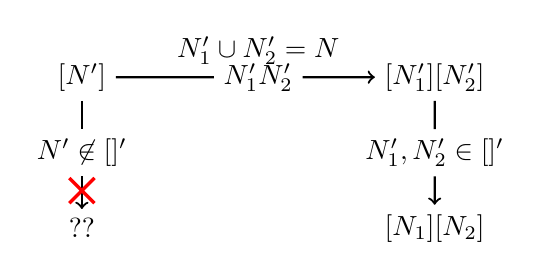
\begin{tikzpicture}[scale=0.8]
            \pgfmathsetmacro{\hs}{1.4};
            \pgfmathsetmacro{\vs}{0.6};
            \pgfmathsetmacro{\cross}{0.2};
            \draw (0*\hs, 4*\vs) node[](a){$\prob[N']$};
            \draw (0*\hs, 2*\vs) node[](ab){$N' \not \in \Inj[\graph]{\graph'}$};
            \draw (4*\hs, 4*\vs) node[](c){$\prob[N_1']\prob[N_2']$};
            \draw (2*\hs, 4*\vs) node[](ac){$N_1' \ancestralindep N_2'$};
            \draw (2*\hs, 4*\vs + 0.7*\vs) node[]{$N_1' \cup N_2' = N$};
            \draw (4*\hs, 2*\vs) node[](cd){$N_1', N_2' \in \Inj[\graph]{\graph'}$};
            \draw (4*\hs, 0*\vs) node[](d){$\prob[N_1]\prob[N_2]$};
            \draw (0, 0) node[](b){??};
            \draw[thick, ] (a) -- (ab);
            \draw[thick, ] (c) -- (cd);
            \draw[thick, ] (a) -- (ac);
            \draw[thick, ->] (ac) -- (c);
            \draw[thick, ->] (ab) -- (b);
            \draw[thick, ->] (cd) -- (d);
            \draw[very thick, red]
            (+ \cross, 1*\vs + \cross) -- (- \cross, 1*\vs - \cross)
            (+ \cross, 1*\vs - \cross) -- (- \cross, 1*\vs + \cross)
            ;
        \end{tikzpicture}
    \end{center}

    Not all sets $N' \subseteq \nodes'$ can be written as the disjoint union of injectable sets, but those that can are called the \term{pre-injectable sets}. A set $N' \subseteq \nodes'$ is a pre-injectable set if it can be decomposed into the disjoint union of injectable sets $N' = \coprod_{i} N'_i \mid N'_i \in \Inj[\graph]{\graph'}$ and all pairs $N_i', N_j'$ are ancestrally independent: $\forall i, j : N_i' \ancestralindep N_j'$.\\

    A pre-injectable set $N'$ is of primal importance to the inflation technique because any distribution over $N'$ will factorize according to graphical $d$-separation conditions~\cite{Pearl_2009},
    \[ \prob[N'] = \prob[\coprod_i N'_i] = \prod_{i}\prob[N'_i] \]
    Application of the inflation lemma to linear inequalities constraining pre-injectable distributions $\prob[N']$ transforms those inequalities into polynomial inequalities over the injectable distributions, allowing one to replace all terms with probability distributions defined over variables in $\nodes$. Throughout the body of this work, we let $\PreInj[\graph]{\graph'}$ denote the set of all pre-injectable sets. Naturally, the pre-injectable sets will define a marginal scenario $\mscenario$ that in \cref{sec:deriving_inequalities} will be used to derive compatibility inequalities\footnote{Analogously for a marginal scenario $\mscenario$, the pre-injectable sets $\PreInj[\graph]{\graph'}$ form an \textit{abstract simplicial complex}. Therefore, in practice, it is completely sufficient to focus on the maximal pre-injectable sets}.

    \begin{center}
    \begin{figure}
    \begin{subfigure}[b]{.45\linewidth}
    \scalebox{1}{\newcommand{\ift}{2.3}
\begin{tikzpicture}[scale=2]
    \begin{scope}[every node/.style=observed]
        \node (C1) at ({-2 + 3*1/\ift}, {3*1/(\ift*sqrt(3))}) {$\p{C}_1$};
        \node (B1) at ({2 - 3*1/\ift}, {3*1/(\ift*sqrt(3))}) {$\p{B}_1$};
        \node (A1) at (0, {2*sqrt(3) - 2*2/sqrt(3)*(1/\ift)}) {$\p{A}_1$};
    \end{scope}
    \begin{scope}[every node/.style=latent]
        \node (X1) at ({-1 + 1/\ift}, {sqrt(3) - 1/(\ift*sqrt(3))}) {$\p{X}_1$};
        \node (Y2) at (1, {sqrt(3)}) {$\p{Y}_2$};
        \node (Y1) at ({1 - 1/\ift}, {sqrt(3) - 1/(\ift*sqrt(3))}) {$\p{Y}_1$};
        \node (Z1) at (0, 0.5) {$\p{Z}_1$};
    \end{scope}
    \begin{scope}[every path/.style={draw=cause, thick}]
        \path[postaction={on each segment={mid arrow}}]
        (X1) -- (A1) (X1) -- (C1)
        (Y2) -- (A1) (Y1) -- (B1)
        (Z1) -- (B1) (Z1) -- (C1)
        ;
    \end{scope}
\end{tikzpicture}}
    \caption{The Cut inflation}\label{fig:cut_inflation}
    \end{subfigure}
    \begin{subfigure}[b]{.45\linewidth}
    \scalebox{1}{\newcommand{\ift}{2.3}
\begin{tikzpicture}[scale=2]
    \begin{scope}[every node/.style=observed]
        \node (C2) at ({-2 + 2*1/\ift}, {2*1/(\ift*sqrt(3))}) {$\p{C}_2$};
        \node (C1) at ({-2 + 3*1/\ift}, {3*1/(\ift*sqrt(3))}) {$\p{C}_1$};
        \node (B2) at ({2 - 2*1/\ift}, {2*1/(\ift*sqrt(3))}) {$\p{B}_2$};
        \node (B1) at ({2 - 3*1/\ift}, {3*1/(\ift*sqrt(3))}) {$\p{B}_1$};
        \node (A2) at (0, {2*sqrt(3) - 2*2/sqrt(3)*(1/\ift)}) {$\p{A}_2$};
        \node (A1) at (0, {2*sqrt(3) - 3*2/sqrt(3)*(1/\ift)}) {$\p{A}_1$};
    \end{scope}
    \begin{scope}[every node/.style=latent]
        \node (X2) at (-1, {sqrt(3)}) {$\p{X}_2$};
        \node (X1) at ({-1 + 1/\ift}, {sqrt(3) - 1/(\ift*sqrt(3))}) {$\p{X}_1$};
        \node (Y2) at (1, {sqrt(3)}) {$\p{Y}_2$};
        \node (Y1) at ({1 - 1/\ift}, {sqrt(3) - 1/(\ift*sqrt(3))}) {$\p{Y}_1$};
        \node (Z1) at (0, 0.5) {$\p{Z}_1$};
        \node (Z2) at (0, 0) {$\p{Z}_2$};
    \end{scope}
    \begin{scope}[every path/.style={draw=cause, thick}]
        \path[postaction={on each segment={mid arrow}}]
        (X1) -- (A1) (X1) -- (C1) (X2) -- (C2) (X1) -- (A2)
        (Y1) -- (A1) (Y1) -- (B1) (Y2) -- (A2) (Y1) -- (B2)
        (Z1) -- (B1) (Z1) -- (C1) (Z2) -- (B2) (Z1) -- (C2)
        ;
    \end{scope}
\end{tikzpicture}}
    \caption{The Spiral inflation}\label{fig:spiral_inflation}
    \end{subfigure}

    \begin{subfigure}[b]{.45\linewidth}
    \scalebox{1.0}{\newcommand{\ift}{2.3}
\newcommand{\hvspoke}{0.8}
\newcommand{\diagspoke}{1.1}
\begin{tikzpicture}[scale=2]
    \begin{scope}[every node/.style=observed]
        \node (A1) at ({0}, {\hvspoke}) {$\p{A}_1$};
        \node (A2) at ({0}, {-\hvspoke}) {$\p{A}_2$};
        \node (B1) at ({-\hvspoke}, {0}) {$\p{B}_1$};
        \node (B2) at ({\hvspoke}, {0}) {$\p{B}_2$};
        \node (C1) at ({+\diagspoke}, {+\diagspoke}) {$\p{C}_1$};
        \node (C2) at ({+\diagspoke}, {-\diagspoke}) {$\p{C}_2$};
        \node (C3) at ({-\diagspoke}, {-\diagspoke}) {$\p{C}_3$};
        \node (C4) at ({-\diagspoke}, {+\diagspoke}) {$\p{C}_4$};
    \end{scope}
    \begin{scope}[every node/.style=latent]
        \node (Y1) at (0, 0) {$\p{Y}_1$};
        \node (X1) at ({0}, {2*\hvspoke}) {$\p{X}_1$};
        \node (Z1) at ({2*\hvspoke}, {0}) {$\p{Z}_1$};
        \node (X2) at ({0}, {-2*\hvspoke}) {$\p{X}_2$};
        \node (Z2) at ({-2*\hvspoke}, {0}) {$\p{Z}_2$};
    \end{scope}
    \begin{scope}[every path/.style={draw=cause, thick}]
        \path[postaction={on each segment={mid arrow}}]
        % Y1
        (Y1) -- (A1)
        (Y1) -- (A2)
        (Y1) -- (B1)
        (Y1) -- (B2)
        % X1
        (X1) -- (C1)
        (X1) -- (C4)
        (X1) -- (A1)
        % Z1
        (Z1) -- (C1)
        (Z1) -- (C2)
        (Z1) -- (B2)
        % X2
        (X2) -- (C2)
        (X2) -- (C3)
        (X2) -- (A2)
        % Z2
        (Z2) -- (C4)
        (Z2) -- (C3)
        (Z2) -- (B1)
        ;
    \end{scope}
\end{tikzpicture}}
    \caption{The Wagon-Wheel inflation}\label{fig:wagon_wheel_inflation}
    \end{subfigure}
    \begin{subfigure}[b]{.45\linewidth}
    \scalebox{1}{\newcommand{\ift}{2.3}
\begin{tikzpicture}[scale=2]
    \begin{scope}[every node/.style=observed]
        \node (C4) at (-2, 0) {$C_4$};
        \node (C3) at ({-2 + 1/\ift}, {1/(\ift*sqrt(3))}) {$C_3$};
        \node (C2) at ({-2 + 2*1/\ift}, {2*1/(\ift*sqrt(3))}) {$C_2$};
        \node (C1) at ({-2 + 3*1/\ift}, {3*1/(\ift*sqrt(3))}) {$C_1$};
        \node (B4) at (2, 0) {$B_4$};
        \node (B3) at ({2 - 1/\ift}, {1/(\ift*sqrt(3))}) {$B_3$};
        \node (B2) at ({2 - 2*1/\ift}, {2*1/(\ift*sqrt(3))}) {$B_2$};
        \node (B1) at ({2 - 3*1/\ift}, {3*1/(\ift*sqrt(3))}) {$B_1$};
        \node (A4) at (0, {2*sqrt(3)}) {$A_4$};
        \node (A3) at (0, {2*sqrt(3) - 2/sqrt(3)*(1/\ift)}) {$A_3$};
        \node (A2) at (0, {2*sqrt(3) - 2*2/sqrt(3)*(1/\ift)}) {$A_2$};
        \node (A1) at (0, {2*sqrt(3) - 3*2/sqrt(3)*(1/\ift)}) {$A_1$};
    \end{scope}
    \begin{scope}[every node/.style=latent]
        \node (X2) at (-1, {sqrt(3)}) {$X_2$};
        \node (X1) at ({-1 + 1/\ift}, {sqrt(3) - 1/(\ift*sqrt(3))}) {$X_1$};
        \node (Y2) at (1, {sqrt(3)}) {$Y_2$};
        \node (Y1) at ({1 - 1/\ift}, {sqrt(3) - 1/(\ift*sqrt(3))}) {$Y_1$};
        \node (Z1) at (0, 0.5) {$Z_1$};
        \node (Z2) at (0, 0) {$Z_2$};
    \end{scope}
    \begin{scope}[every path/.style={draw=cause, thick}]
        \path[postaction={on each segment={mid arrow}}]
        (X2) -- (A4) (X2) -- (C4) (X2) -- (C2) (X2) -- (A3)
        (Y2) -- (A4) (Y2) -- (B4) (Y2) -- (A2) (Y2) -- (B3)
        (Z2) -- (B4) (Z2) -- (C4) (Z2) -- (B2) (Z2) -- (C3)
        (X1) -- (A1) (X1) -- (C1) (X1) -- (C3) (X1) -- (A2)
        (Y1) -- (A1) (Y1) -- (B1) (Y1) -- (A3) (Y1) -- (B2)
        (Z1) -- (B1) (Z1) -- (C1) (Z1) -- (B3) (Z1) -- (C2)
        ;
    \end{scope}
\end{tikzpicture}}
    \caption{The Web Inflation}\label{fig:the_web_inflation}
    \end{subfigure}
    \caption{Some inflations of the triangle scenario.}
    \label{fig:inflations}
    \end{figure}
    \end{center}

    \section{Deriving Inequalities}
    \label{sec:deriving_inequalities}

    In \cref{sec:causal_compatibility}, we defined the notion of a causal compatibility inequality without providing a means for deriving/computing them. This section aims to delineate algorithms and methods that can be used to derive causal compatibility inequalities for generic causal inference problems. Recalling the definition of causal compatibility presented in \cref{sec:compatibility}, a marginal model $\prob^{\mscenario}$ is compatible with a causal structure $\graph = \br{\nodes, \edges}$ if it can be recovered from a series of operations. First choose a set of causal parameters $\bc{\prob[n\mid\Pa[\graph]{n}] \mid n \in \nodes}$ and then construct a joint distribution $\prob[\nodes] = \prod_{n \in \nodes} \prob[n \mid \Pa[\graph]{n}]$ over all nodes $\nodes$ (this step is \cref{eq:local_markov_property_operation}). Afterwards, each marginal distribution $\prob[V] \in \mscenario$ should be recoverable from a marginalization over $\prob[\nodes]$ (this step is the combination of \cref{eq:observable_marginalization,eq:context_marginalization}). Intuitively, these two requirements for a compatible marginal model $\prob^{\mscenario}$ provide two necessary components of compatibility:
    \begin{enumerate}
        \item The marginal model $\prob^{\mscenario}$ must admit a joint distribution $\prob[\nodes]$ (\cref{eq:observable_marginalization,eq:context_marginalization}).
        \item The joint distribution $\prob[\nodes]$ must satisfy the Markov separability criteria (\cref{eq:local_markov_property_operation}).
    \end{enumerate}
    In practice, this is the natural order in which to classify the compatibility of a marginal model $\prob^{\mscenario}$. First check if the marginal model admits a joint distribution and if and only if it does, determine whether or not the local Markov property can be satisfied for some choice of causal parameters. Intuitively, there are two reasons why a given marginal model $\prob^{\mscenario}$ would be deemed incompatible. One possibility is that the marginal model $\prob^{\mscenario}$ does not admit a joint distribution $\prob[\nodes]$. Alternatively, it could be possible that a joint distribution $\prob[\nodes]$ exists but can not factor into causal parameters as per \cref{eq:local_markov_property_operation}.\\

    Colloquially, the first necessary condition, namely the existence (or non-existence) of a joint distribution, is referred to as \term{the marginal problem}. The marginal problem asks: given a marginal model $\prob^{\mscenario} = \bc{\prob[V] \mid V \in \mscenario}$ marginal to the joint variables $\jointvar = \bigcup_{V \in \mscenario} V$, does there exist a joint distribution $\prob[\jointvar]$ such that each context $\prob[V]$ can be obtained by marginalizing $\prob[\jointvar]$?
    \[ \forall V \in \mscenario : \prob[V] = \sum_{\jointvar \setminus V} \prob[\jointvar] \eq \label{eq:def:marginal_problem}\]
    Note that we have changed notation from the nodes of a causal structure $\nodes$ to a joint set of variables $\jointvar$. This is done simply because the marginal problem is well-defined independent of a given causal structure. In fact, if a marginal model $\prob^{\mscenario}$ does not admit a joint distribution, then it cannot be compatible with \textit{any} causal structure whatsoever. A marginal model is said to be \textit{contextual} if it \textit{does not} admit a joint distribution and \textit{non-contextual} otherwise. The marginal problem has applications to numerous areas of mathematics including game theory~\cite{Vorobev_1962}, database theory, knowledge integration of expert system, and of course, quantum information theory~\cite{Fritz_2011}. \\

    The marginal problem is distinct from the second necessary condition, which we term the \term{Markov separability problem} in numerous ways. First of all, the marginal problem as applied to causal inference tasks is only concerned with the observable variables $\nodes_{O}$ of $\graph$. This differs from the Markov separability problem which depends directly on the entire graphical structure of $\graph$ and thus must include the latent variables $\nodes_{L}$. The purpose of latent variables is to have unspecified behavior which makes checking the local Markov property exceedingly difficult in comparison to the marginal problem. Secondly, \cref{eq:def:marginal_problem} is inherently a linear system of constraints which be solved rather efficiently using linear programs (to be discussed in \cref{sec:marginal_linear}). The local Markov property concerns itself with probabilistic independence constraints which are polynomial. Fortunately, the Inflation Technique (summarized in \cref{sec:inflation_technique}) is able to cast (at least partially) the Markov separability problem as a marginal problem over an inflated causal structure. As such the Inflation Technique in many ways can be considered a relaxation technique which turns polynomial constraints into linear constraints. \\

    In consideration of these observations, we will now endeavor to discuss how causal compatibility inequalities can be derived by casting the marginal problem as a linear program. After doing, it becomes possible to discuss existing methods for deriving constraints on the set of contextual marginal models.

    \subsection{The Marginal Problem as a Linear Program}
    \label{sec:marginal_linear}

    Heretofore, our discussions of compatibility and the marginal problem have been general in the sense of making no reference to the nature the random variables $v \in \jointvar$. In particular, whether the outcomes of $v$ are discrete or continuous, finite or unbounded, or otherwise. In the case of infinite outcomes, the marginal problem can be used to derive entropic inequalities defined over the mutual information between variables $v \in \jointvar$~\cite{Fritz_2011}. Entropic inequalities however have been shown to be less constraining than inequalities defined over variables with finite cardinality~\cite{Inflation}. Throughout this document, we restrict our attention to finite outcomes. To assist with the subsequent analysis, we recall some familiar notions of probability theory.

    \subsubsection{Events \& Outcomes}
    To every discrete random variable $v$ there corresponds a prescribed set of \term{outcomes} $O_v$. We also define the set of all \term{events over $v$} $\Events{v}$\footnote{In the language of sheaf-theory, $\Events{v}$ is the \textit{sheaf of events}~\cite{Abramsky_2011}.} to be the set of all functions $s : \bc{v} \to O_v$ each representing the event that a measurement on $v$ was made where $s\br{v} \in O_v$ was observed.
    \[ \Events{v} \defined \bc{s : \bc{v} \to O_v} \]
    Evidently, $\Events{v}$ and $O_v$ have a one-to-one correspondence and this distinction can be confounding. There is rarely any harm in referring synonymously to either as outcomes. Nonetheless, a sheaf-theoretic treatment of contextuality~\cite{Abramsky_2011} demands the distinction.
    Specifically for this work, the distinction becomes essential for our discussion and exploit of marginal symmetries in \cref{sec:symmetric_inequalities}. As a natural generalization we define the event over a collection of random variables $V = \bc{v_1, \ldots, v_n}$ in a parallel manner,
    \[ \Events{V} \defined \bc{s: V \to O_{V} \mid \forall i : s\br{v_i} \in O_{v_i} } \eq \label{eq:outcome_space}\]
    Each event $s$ can be compactly represented as a set of mappings over each element of $V$.
    \[ s = \bc{v_1 \mapsto s\br{v_1}, \ldots, v_k \mapsto s\br{v_k}} = \bc{v_i\mapsto s\br{v_i}}_{i = 1}^{k} \]
    The domain $\Dom{s}$ of an event $s$ is the set of random variables it valuates, i.e. if $s \in \Events{V}$, then $\Dom{s} = V$. Under this framework, a probability distribution $\prob[V]$ can be considered as a map from $\Events{V}$ to the unit interval $\bs{0,1}$.
    \begin{example}
        Let $s \in \Events{V}$ be an event over $V$, a probability distribution $\prob[V]$ over $V$ will assign a non-negative probability $\prob[V][s]$ to $s$. Let $V = \bc{v_1, v_2}$ with each $v \in V$ having $3$ distinct outcomes $O_v = \bc{0,1,2}$. Furthermore let $f \in \Events{V}$ be the event $\br{v_1 \mapsto 2, v_2 \mapsto 1}$. The following notations are interchangeable,
        \[ \prob[][s] = \prob[\Dom{s}][s] = \prob[V][s] = \prob[v_1, v_2][s] = \prob[][v_1 \mapsto s_1\br{v_1}, v_2 \mapsto s_2\br{v_2}] = \prob[][v_1 = 2, v_2 = 1] = \prob[v_1v_2][21] \]
        Each of which should be read as ``the probability that $v_1$ got outcome $2$ and $v_2$ got outcome $1$''
    \end{example}
    The marginal problem inherently depends on the concept of probabilistic marginalization. This concept can be understood at the level of events; one event $s \in \Events{V}$ can be ``marginalized'' or restricted to a smaller event $s' \in \Events{W}$ whenever $W \subseteq V$.
    \begin{definition}
    \label{def:section_restriction}
    For every $W \subseteq V$ and $s \in \Events{V}$, the \term{restriction of $s$ onto $W$} (denoted $s|_{W} \in \Events{W}$) is the event in $\Events{W}$ that \textit{agrees} with each of $s$'s assignments for variables in $W$.
    \[ \forall v \in W : s|_{W}\br{v} = s\br{v} \]
    \end{definition}
    % \begin{definition}
    % \label{def:section_compatible}
    % The events $s_{V} \in \Events{V}$ and $s_{W} \in \Events{W}$ are said to be \term{compatible} events if they agree on their valuations of $V \cap W$. Compatibility will be denoted with the infix `$\com$'.
    % \[ s_{V} \com s_{W} \iff {s_{V}}|_{V\cap W} = {s_{W}}|_{V\cap W} \]
    % \end{definition}
    % \begin{definition}
    % \label{def:section_extendable}
    % It $s_V \in \Events{V}$ and $s_W \in \Events{W}$ compatible events and $W \subseteq V$ then $s_W$ is said to be \term{extendable} to $s_V$. Extendability will be denoted with the infix `$\ext$'.
    % \[ s_W \ext s_V \iff s_W \com s_V, W \subseteq V \]
    % Extendability is dual to the notion of a \term{restriction} of $s_V$; $s_V$ can be restricted to $s_W$ ($s_V \res s_W$) if and only if $s_W$ is extendable to $s_V$.
    % \end{definition}

    % \begin{remark}
    %     The notation `$s \com t$' is used to indicate compatibility between $s \in \Events{V}$ and $t \in \Events{W}$ because of the following observation: $s$ and $t$ are compatible if and only if they are extensions of some event $r \in \Events{V \cap W}$.
    %     \[ s \com t \iff \exists r \in \Events{V \cap W} \mid s \res r \ext t \]
    %     In fact $r$ is uniquely defined.
    %     \[ \forall v \in V \cap W : r\br{v} = s\br{v} = t\br{v} \]
    % \end{remark}

    For every marginal scenario $\mscenario = \bc{V_1, \ldots, V_k}$, it is useful to put special emphasis on the \term{joint events} $\Events{\jointvar}$ which represent all possible global events over the entire set of joint variables. Similarly, we define the \term{context events} for a particular context $V \in \mscenario$ as $\Events{V}$. Finally, we elect to define the \term{marginal events} as the disjoint union of all context events and by an abuse of notation we will denote this disjoint union as $\Events{\mscenario}$.
    \[ \Events{\mscenario} = \coprod_{V \in \mscenario} \Events{V} \]
    Each marginal section $m \in \Events{\mscenario}$ has a domain $\Dom{m} = V$ for some $V \in \mscenario$. By construction each marginal event $m \in \Events{\mscenario}$ is a restriction of some joint event $j \in \Events{\jointvar}$.
    \subsubsection{Linear Programs}
    \label{sec:linear_programs}
    The marginalization operation (\cref{eq:def:marginal_problem}) of the marginal problem is a linear operator. This linear operator maps a joint probability distribution $\prob[\jointvar] : \Events{\jointvar} \to \bs{0,1}$ into a marginal model $\prob^{\mscenario} = \bc{\prob[V] : \Events{V} \to \bs{0,1} \mid V \in \mscenario}$. Since $\Events{\mscenario}$ and $\Events{\jointvar}$ are finite, the marginal problem can be casted as a $\abs{\Events{\mscenario}} \times \abs{\Events{\jointvar}}$ matrix.

    \begin{definition}
        \label{def:incidence_matrix}
        The \term{incidence matrix} $M$ for a marginal scenario $\mscenario = \bc{V_1, \dots, V_k}$ is a bit-wise matrix where the columns are indexed by \textit{joint} events $j \in \Events{\jointvar}$ and the rows are events by \textit{marginal} events $m \in \Events{\mscenario}$. The entries of $M$ are populated whenever a marginal event $m$ is a restriction of the joint event $j$.
        \[ M_{m,j} \defined \begin{cases}
            1 & m = j|_{\s{D}\br{m}} \\
            0 & \text{otherwise}
        \end{cases} \]
        The incidence matrix has $\abs{\Events{\jointvar}}$ columns, $\abs{\Events{\mscenario}} = \sum_{i} \abs{\Events{V_i}}$ rows and $k\abs{\Events{\jointvar}}$ non-zero entries.
    \end{definition}
    To illustrate this concretely, consider the following example:
    \begin{example}
        \label{ex:incidence_matrix}
        Let $\jointvar$ be $3$ binary variables $\jointvar = \bc{A,B,C}$ and $\mscenario$ be the marginal scenario $\mscenario = \bc{\bc{A,B}, \bc{B,C}, \bc{A,C}}$. The incidence matrix becomes:
        \[ M = \kbordermatrix{
            (A,B,C) \:\: \mapsto & (0,0,0) & (0,0,1) & (0,1,0) & (0,1,1) & (1,0,0) & (1,0,1) & (1,1,0) & (1,1,1) \\
            (A\mapsto0, B\mapsto0) & \kone & \kone & \kzer & \kzer & \kzer & \kzer & \kzer & \kzer \\
            (A\mapsto0, B\mapsto1) & \kzer & \kzer & \kone & \kone & \kzer & \kzer & \kzer & \kzer \\
            (A\mapsto1, B\mapsto0) & \kzer & \kzer & \kzer & \kzer & \kone & \kone & \kzer & \kzer \\
            (A\mapsto1, B\mapsto1) & \kzer & \kzer & \kzer & \kzer & \kzer & \kzer & \kone & \kone \\
            (B\mapsto0, C\mapsto0) & \kone & \kzer & \kzer & \kzer & \kone & \kzer & \kzer & \kzer \\
            (B\mapsto0, C\mapsto1) & \kzer & \kone & \kzer & \kzer & \kzer & \kone & \kzer & \kzer \\
            (B\mapsto1, C\mapsto0) & \kzer & \kzer & \kone & \kzer & \kzer & \kzer & \kone & \kzer \\
            (B\mapsto1, C\mapsto1) & \kzer & \kzer & \kzer & \kone & \kzer & \kzer & \kzer & \kone \\
            (A\mapsto0, C\mapsto0) & \kone & \kzer & \kone & \kzer & \kzer & \kzer & \kzer & \kzer \\
            (A\mapsto0, C\mapsto1) & \kzer & \kone & \kzer & \kone & \kzer & \kzer & \kzer & \kzer \\
            (A\mapsto1, C\mapsto0) & \kzer & \kzer & \kzer & \kzer & \kone & \kzer & \kone & \kzer \\
            (A\mapsto1, C\mapsto1) & \kzer & \kzer & \kzer & \kzer & \kzer & \kone & \kzer & \kone
        } \eq \label{eq:example_incidence}\]
    \end{example}
    The incidence matrix needs to act (to the right) on a vector representing the joint probability $\prob[\jointvar]$ distribution and output a vector representing the marginal model $\prob^{\mscenario}$.
    \begin{definition}
        The \term{joint distribution vector} $\probvec^{\jointvar}$ for a probability distribution $\prob[\jointvar]$ is the vector whose entries are the positive, real-valued probabilities that $\prob[\jointvar]$ assigns to each joint event $j \in \Events{\jointvar}$. $\probvec^{\jointvar}$ shares the same indices as the \textit{column} indices of $M$.
        \[ \forall j \in \Events{\jointvar} : \probvec^{\jointvar}_j = \prob[\jointvar][j] \]
    \end{definition}
    \begin{definition}
        Analogously, \term{marginal distribution vector} $\probvec^{\mscenario}$ for a marginal model $\prob^{\mscenario} = \bc{P_{V_1}, \ldots, P_{V_k}}$ is the vector whose entries are probabilities over the set of marginal outcomes $\Events{\mscenario}$. $\probvec^{\mscenario}$ shares the same indices as the \textit{row} indices of $M$.
        \[ \forall m \in \Events{\mscenario} : \probvec^{\mscenario}_m = \prob[\Dom{m}][m] \]
    \end{definition}
    By design, the marginal and joint distribution vectors are related via the incidence matrix $M$. Given a joint distribution vector $\probvec^{\jointvar}$ one can obtain the marginal distribution vector $\probvec^{\mscenario}$ by multiplying $M$ by $\probvec^{\jointvar}$.
    \[ \probvec^{\mscenario} = M \tcdot \probvec^{\jointvar} \eq \label{eq:incidence_matrix_use} \]
    Because the marginal distribution vector $\probvec^{\mscenario}$ is simply another representation of the marginal model $\prob^{\mscenario}$, we will henceforth use the language interchangeably. This is likewise done so for the joint distribution (vector) $\prob[\jointvar]$ ($\probvec^{\jointvar}$). As a quick remark, the particular ordering of the rows and columns of $M$ carries \textit{no importance}, but it \textit{must} be consistent between $M$, $\probvec^{\jointvar}$ and $\probvec^{\mscenario}$. The marginal problem can now be rephrased in the language of the incidence matrix. Suppose one obtains a marginal distribution vector $\probvec^{\mscenario}$; the marginal problem becomes equivalent to the question:
    \textit{Does there exist a joint distribution vector $\probvec^{\jointvar}$ such that \cref{eq:incidence_matrix_use} holds?} \\

    The marginal problem can sometimes take on a more general variant that does not begin with a specific marginal model~\cite{Abramsky_2012,Mansfield_2012,Fritz_2011}: \textit{Given a marginal scenario $\mscenario$, what is the set of all non-contextual marginal models?} \citet{Pitowsky_1991} demonstrates that the set of non-contextual marginal models forms a \textit{convex} polytope called the \term{marginal polytope}. The extremal rays of a marginal polytope directly correspond to the columns of $M$ which correspond to each of the $\abs{\Events{\jointvar}}$ \textit{deterministic} joint distributions $\probvec^{\jointvar}$. Since all joint distributions $\probvec^{\jointvar}$ are probability distributions, their entries must sum to unity.
    \[ \sum_{j \in \Events{\jointvar}} \probvec^{\jointvar}_j = 1 \]
    This normalization defines the convexity of the polytope; all non-contextual marginal models are convex mixtures of the deterministic marginal models pursuant to \cref{eq:incidence_matrix_use}. The marginal polytope is a beneficial tool for understanding contextuality. First, the \textit{facets} of a marginal polytope correspond to a finite set of linear inequalities that are complete in the sense that all contextual distributions violate at least one facet inequality~\cite{Brunner_2013}. From the perspective of a marginal polytope, convex hull algorithms can be used to compute a representation of the complete set of linear inequalities and completely solve the marginal problem. Alternatively, one can completely characterize the separation between the space of contextual and non-contextual distributions by the system of inequalities associated with \cref{eq:incidence_matrix_use}. Explicitly,
    \begin{equation} \label{eq:halfspace_rep_incidence}
    \begin{alignedat}{2}
        \forall m \in \Events{\mscenario} :&&\quad \probvec^{\mscenario}_m - {\sum}_{j} M_{m, j} \probvec^{\jointvar}_j &\geq 0 \\
        \forall m \in \Events{\mscenario} :&&\quad -\probvec^{\mscenario}_m + {\sum}_{j} M_{m, j} \probvec^{\jointvar}_j &\geq 0 \\
        \forall j \in \Events{\jointvar} :&&\quad \probvec^{\jointvar}_j &\geq 0
    \end{alignedat}
    \end{equation}
    Geometrically \cref{eq:halfspace_rep_incidence} is a family of $2\abs{\Events{\mscenario}} + \abs{\Events{\jointvar}}$ half-planes bounding $\R^{\abs{\Events{\mscenario}}} \times \R^{\abs{\Events{\jointvar}}}$. However testing the contextuality of a marginal model $\probvec^{\mscenario}$ requires a collection of inequalities bounding just $\R^{\abs{\Events{\mscenario}}}$. Transforming \cref{eq:halfspace_rep_incidence} into the desired system of inequalities is the task of linear-quantifier elimination. A popular tool for linear quantifier elimination is \term{Fourier-Motzkin elimination} \cite{Dantzig_1973,Inflation,Abramsky_2012,jones_2004}. Applying the Fourier-Motzkin procedure to completely solve the marginal problem is discussed in more detail in \citet{Fritz_2011}. An excellent survey of existing techniques for solving the marginal problem including Equality Set Projection~\cite{jones_2004} and Hardy-type hypergraph transversals can be found in \citet{Inflation}. In conclusion, there are a number of computational tools available to solve the marginal problem completely whenever no marginal model is provided. \\

    Each of the above mentioned techniques suffers from computational complexity limitations. For example, the Fourier-Motzkin procedure is act worst case doubly exponential in the number of initial inequalities~\cite{Dantzig_1973}. For the purposes of this research, solving the marginal problem without reference to a marginal model was intractable. This will become apparent in \cref{sec:found_inequalities} when the inflation technique is applied to the triangle scenario, producing marginal models that are very large. Moreover, algorithms to partially solve the marginal problem such as Hardy-type hypergraph transversals were used to determine hundreds of thousands of causal compatibility inequalities for the triangle scenario; none of which were able to be violated quantumly using numerical optimizations. Therefore, simpler approaches to the marginal problem needed to be considered. \\

    Luckily, the Fritz distribution (\cref{sec:fritz_distribution}) allows one to avoid the complexity issues of the complete marginal problem and instead focus on the original problem of determining where or not a particular marginal model admitted a joint distribution or not. This question is naturally framed as the following linear problem:

    \begin{definition}
        \label{def:marginal_linear_program}
        \term{The Marginal Linear Program} is the following linear program:
        \begin{alignat*}{2}
            & \text{minimize:} \quad&& \emptyset \tcdot x\\
            & \text{subject to:} && x \succeq 0 \\
            & && M \tcdot x = \probvec^{\mscenario}
        \end{alignat*}
        If this ``optimization''\footnote{``Optimization'' is presented in quotes here because the minimization objective is trivially always zero ($\emptyset$ denotes the null vector of all zero entries). The primal value of the linear program is of no interest, all that matters is its \textit{feasibility}.} is \textit{feasible}, then there exists a vector $x$ than can satisfy \cref{eq:incidence_matrix_use} and is a valid joint distribution vector. Therefore feasibility implies that $\probvec^{\jointvar}$ exists and is precisely $x$. Moreover if the marginal linear program is \textit{infeasible}, then there \textit{does not} exist a joint distribution $\probvec^{\jointvar}$.
    \end{definition}

    To every linear program, there exists a dual linear program that characterizes the feasibility of the original~\cite{Schrijver_1998}. Constructing the dual linear program is straightforward~\cite{Lahaie_2008}.

    \begin{definition}
        \label{def:dual_marginal_linear_program}
        \term{The Dual Marginal Linear Program}:
        \begin{alignat*}{2}
            & \text{minimize:} \quad&& y \tcdot \probvec^{\mscenario}\\
            & \text{subject to:} && y \tcdot M \succeq 0
        \end{alignat*}
        Where $y$ is a real valued vector with the same length as $\probvec^{\mscenario}$.
    \end{definition}

    The dual marginal linear program not only answers the marginal problem for a specific marginal model $\probvec^{\mscenario}$ but as a by-product provides an inequality that witnesses its contextuality. If this is not obvious, first notice that the dual problem is \textit{never infeasible}; by choosing $y$ to be trivially the null vector $\emptyset$ of appropriate size, all constraints become satisfied. Secondly if the dual constraint $y \tcdot M \succeq 0$ holds \textit{and} the primal is feasible, then the following must hold:
    \[ y \tcdot \probvec^{\mscenario} =  y \tcdot M \tcdot x \geq 0 \eq \label{eq:dual_marginal_ineq} \]
    Therefore the \textit{sign} of the dual objective $d \defined \min \br{y \tcdot \probvec^{\mscenario}}$ classifies a marginal model's contextuality. If $d < 0$ then \cref{eq:dual_marginal_ineq} is violated and therefore $\probvec^{\mscenario}$ is contextual. Likewise if $d \geq 0$ (satisfying \cref{eq:dual_marginal_ineq}), then $\probvec^{\mscenario}$ is non-contextual.\footnote{Actually, if $d \geq 0$ then it is exactly $d = 0$ due to the existence of the trivial $y = \emptyset$. This observation is an instance of the \textit{Complementary Slackness Property} of~\cite{Bradley_1977}. Moreover, if $d < 0$, then it is unbounded $d = -\inf$. This latter point becomes clear upon recognizing that for any $y$ with $d < 0$, another $y' = \al y$ can be constructed (with $\al > 1$) such that $d' = \al d < d$. Since a more negative $d'$ can always be found, it must be that $d$ is unbounded. This is a demonstration of the fundamental \textit{Unboundedness Property} of~\cite{Bradley_1977}; if the dual is unbounded, then the primal is infeasible.} This is manifestation of Farkas's lemma~\cite{Schrijver_1998}. \\

    An \term{infeasibility certificate}~\cite{Andersen_2001} is any vector $y$ that satisfies the constraint of \cref{def:dual_marginal_linear_program} and also permits violation of \cref{eq:dual_marginal_ineq} for some marginal distribution vector $\probvec^{\mscenario}$.
    \[ y \in \R^{\abs{\Events{\mscenario}}} : y \tcdot M \succeq 0, \quad y \tcdot \probvec^{\mscenario} < 0 \]
    Most linear program software packages such as Mosek~\cite{Mosek_2016}, Gurobi~\cite{Gurobi_2016}, CPLEX~\cite{Cplex_2016} and CVX/CVX OPT~\cite{CVX_2016,CVX_Opt_2016} are capable of producing infeasibility certificates.
    Furthermore, for every $y$ satisfying $y \tcdot M \succeq 0$ there corresponds a \term{certificate inequality} that constraints the set of non-contextual marginal models. If $y$ is an infeasibility certificate, then all non-contextual marginal models $\probvec^{\mscenario}$ must satisfy \cref{eq:dual_marginal_ineq} making $y \cdot \probvec^{\mscenario} \geq 0$ a valid causal compatibility inequality.

    \subsection{Triangle Scenario Inequalities}
    \label{sec:found_inequalities}

    Equipped with the Fritz distribution (\cref{sec:fritz_distribution}) and the inflation technique (\cref{sec:inflation_technique}), it is now possible to derive causal compatibility inequalities for the triangle that are violated by the Fritz distribution; the procedure for doing so is as follows. First select an inflation $\graph'$ of the triangle scenario $\graph$ and identify the maximal pre-injectable sets $\PreInj[\graph]{\graph'}$. These sets define the marginal scenario to be used in the Inflation Technique. Next, inflate the Fritz distribution into the pre-injectable sets as described by the Inflation lemma (\cref{lem:inflation}). Finally, obtain infeasibility certificates using some linear programing software and obtain a valid causal compatibility inequality that witnesses the Fritz distribution's incompatibility. \\

    As a first demonstration, we make use of the Wagon-Wheel inflation (\cref{fig:wagon_wheel_inflation}) to find these inequalities. The Wagon-Wheel inflation possesses $4$ copies of $C$ ($C_1, C_2, C_3, C_4$) and $2$ copies of $A$ ($A_1, A_2$) and $B$ ($B_1, B_2$) arranged in the shape of a Wagon-Wheel. By inspection\footnote{Computing the injectable and pre-injectable sets computationally is possible and a technique is discussed in~\citet{Inflation}.}, the maximal pre-injectable sets of the Wagon-Wheel inflation are as follows:
    \begin{equation*}
        \eq \label{eq:pre_injectable_triangle_scenario_wagon_wheel}
        \begin{gathered}
            \textbf{Maximal Pre-injectable Sets} \\
            \bc{A_2, B_1, C_3, C_1} \\
            \bc{A_1, B_1, C_4, C_2} \\
            \bc{A_1, B_2, C_1, C_3} \\
            \bc{A_2, B_2, C_2, C_4} \\
        \end{gathered}
        \qquad
        \begin{gathered}
            \textbf{Ancestral Independences} \\
            \bc{A_2, B_1, C_3} \ancestralindep \bc{C_1} \\
            \bc{A_1, B_1, C_4} \ancestralindep \bc{C_2} \\
            \bc{A_1, B_2, C_1} \ancestralindep \bc{C_3} \\
            \bc{A_2, B_2, C_2} \ancestralindep \bc{C_4} \\
        \end{gathered}
    \end{equation*}

    These maximal pre-injectable sets define a marginal scenario where $\graph'$ is the Wagon-Wheel inflation of the triangle scenario $\graph$.
    \[ \mscenario = \PreInj[\graph]{\graph'} = \bc{\bc{A_2, B_1, C_3, C_1}, \bc{A_1, B_1, C_4, C_2}, \bc{A_1, B_2, C_1, C_3}, \bc{A_2, B_2, C_2, C_4}} \eq \label{eq:wagon_wheel_marginal_model}\]
    The complete set of variables $\jointvar$ is simply the set of observable nodes in the Wagon-Wheel inflation,
    \[ \jointvar = \nodes'_O = \bc{A_1, A_2, B_1, B_2, C_1, C_2, C_3, C_4} \]
    Given that the Fritz distribution is defined over $4$-outcomes variables, the variables in the marginal scenario are assigned $4$-outcomes as well. This marginal scenario $\mscenario$ then defines an incidence matrix capable of accommodating the Fritz distribution.
    Analogously to \cref{ex:incidence_matrix}, this marginal scenario defines an incidence matrix $M$ that has $\abs{\Events{\mscenario}} = \sum_{V \in \mscenario} \abs{\Events{V}} = 4 \cdot 4^{4} = 1024$ rows and $\abs{\Events{\jointvar}} = \prod_{v \in \jointvar} \abs{\Events{v}} = 4^{\abs{\jointvar}} = 4^8 = 65,536$ columns. Understandably, this matrix is not reproduced here. The sheer size of the incidence matrix used here makes complete solutions of the marginal problem using tools such as linear-quantifier elimination intractable.\\

    The marginal distribution vector $\probvec^{\mscenario}$ is indexed by $1024$ marginal outcomes $m \in \Events{\mscenario}$ of the following \textit{symbolic} form,
    \[ {\probvec^{\mscenario}}^{\intercal} = \underbrace{\br{\prob[A_2B_1C_3C_1]\br{0000}, \ldots, \prob[A_1B_1C_4C_2]\br{3232}, \ldots, \prob[A_2B_2C_2C_4]\br{3333}}}_{1024 \text{ entries}} \eq \label{eq:marginal_vector_wagon_wheel} \]
    Which can be factored into the ancestrally independent injectable sets using \cref{eq:pre_injectable_triangle_scenario_wagon_wheel},
    \[ {\probvec^{\mscenario}}^{\intercal} = \br{\prob[A_2B_1C_3]\br{000}\prob[C_1]\br{0}, \ldots, \prob[A_1B_1C_4]\br{323}\prob[C_2]\br{2}, \ldots, \prob[A_2B_2C_2]\br{333}\prob[C_4]\br{3}} \eq \label{eq:marginal_vector_wagon_wheel_factors}\]
    And finally, each probability distribution in \cref{eq:marginal_vector_wagon_wheel_factors} is deflated by dropping copy-indices.
    \[ {\probvec^{\mscenario}}^{\intercal} = \br{\prob[ABC]\br{000}\prob[C]\br{0}, \ldots, \prob[ABC]\br{323}\prob[C]\br{2}, \ldots, \prob[ABC]\br{333}\prob[C]\br{3}} \eq \label{eq:marginal_vector_wagon_wheel_factors_dropped}\]
    This step is permitted because all of the remaining distributions in \cref{eq:marginal_vector_wagon_wheel_factors} are defined over the injectable sets of the Wagon-Wheel inflation. Numerically however, each of the elements of $\probvec^{\mscenario}$ are replaced with numerical values corresponding to the Fritz distribution upon deflation. Pursuant to \cref{eq:fritz_dist}, $\prob[ABC]\br{323}\prob[C]\br{2}$, for example, is assigned the following numerical value.
    \[ \prob[ABC]\br{323}\prob[C]\br{2} = \f{1}{32}\br{2 + \sqrt{2}} \cdot \f{1}{4} \simeq 0.0267  \]
    The same is applied to all other entries of $\probvec^{\mscenario}$. Finally, this numerical version of $\probvec^{\mscenario}$ and $M$ are subjected to linear programing software and an infeasibility certificate $y$ was obtained. Below is an example of an infeasibility inequality obtained over the entries of \cref{eq:marginal_vector_wagon_wheel_factors_dropped}.
    \begin{equation*}
    \begin{gathered}
    \eq\label{eq:ww_ineq}
    2P_{ABC}(203)P_{C}(0) + 2P_{ABC}(303)P_{C}(0) + P_{ABC}(003)P_{C}(0) + P_{ABC}(013)P_{C}(0) + \\
    P_{ABC}(020)P_{C}(2) + P_{ABC}(022)P_{C}(2) + P_{ABC}(023)P_{C}(0) + P_{ABC}(023)P_{C}(2) + \\
    P_{ABC}(030)P_{C}(2) + P_{ABC}(031)P_{C}(2) + P_{ABC}(032)P_{C}(2) + P_{ABC}(033)P_{C}(0) + \\
    P_{ABC}(033)P_{C}(2) + P_{ABC}(103)P_{C}(0) + P_{ABC}(113)P_{C}(0) + P_{ABC}(123)P_{C}(0) + \\
    P_{ABC}(133)P_{C}(0) + P_{ABC}(200)P_{C}(0) + P_{ABC}(200)P_{C}(1) + P_{ABC}(200)P_{C}(2) + \\
    P_{ABC}(200)P_{C}(3) + P_{ABC}(201)P_{C}(0) + P_{ABC}(201)P_{C}(1) + P_{ABC}(201)P_{C}(2) + \\
    P_{ABC}(201)P_{C}(3) + P_{ABC}(203)P_{C}(1) + P_{ABC}(203)P_{C}(2) + P_{ABC}(203)P_{C}(3) + \\
    P_{ABC}(213)P_{C}(0) + P_{ABC}(223)P_{C}(0) + P_{ABC}(300)P_{C}(0) + P_{ABC}(300)P_{C}(1) + \\
    P_{ABC}(300)P_{C}(2) + P_{ABC}(300)P_{C}(3) + P_{ABC}(301)P_{C}(0) + P_{ABC}(301)P_{C}(1) + \\
    P_{ABC}(301)P_{C}(2) + P_{ABC}(301)P_{C}(3) + P_{ABC}(302)P_{C}(1) + P_{ABC}(303)P_{C}(1) + \\
    P_{ABC}(303)P_{C}(2) + P_{ABC}(303)P_{C}(3) + P_{ABC}(313)P_{C}(0) - P_{ABC}(000)P_{C}(3) \geq 0
    \end{gathered}
    \end{equation*}
    By construction, every marginal model $\probvec^{\mscenario} = \bc{\prob[ABC], \prob[AB], \prob[BC], \prob[AC], \prob[A], \prob[B], \prob[C]}$ compatible with the triangle scenario must satisfy \cref{eq:ww_ineq}. The Fritz distribution however violates \cref{eq:ww_ineq}.\\

    Notice the final term $\prob[ABC]\br{000}\prob[C]\br{3}$ has a coefficient $-1$. For the Fritz distribution, $\prob[ABC]\br{000}\prob[C]\br{3} = \f{1}{128}\br{2 + \sqrt{2}} \simeq 0.0267$ but all of the remaining terms sum to $\simeq 0.0136$ meaning that the Fritz distribution violates this inequality with violation $-0.0129\ldots \not \geq 0$.


    It is possible to simplify this inequality by marginalizing over sets of terms such as $P_{ABC}(300)P_{C}(0) + P_{ABC}(300)P_{C}(1) + P_{ABC}(300)P_{C}(2) + P_{ABC}(300)P_{C}(3) = P_{ABC}(300)$. Upon doing so, one obtains the following,
    \begin{gather*}
        P_{ABC}(000)P_{C}(3) + P_{ABC}(021)P_{C}(2) + P_{ABC}(202) + P_{ABC}(302) + P_{ABC}(233)P_{C}(0) + P_{AC}(33)P_{C}(0) \leq \\ P_{ABC}(303)P_{C}(0) + P_{ABC}(313)P_{C}(0) + P_{ABC}(302)P_{C}(1) + \\
        + P_{AB}(02)P_{C}(2) + P_{AB}(03)P_{C}(2) + P_{AB}(20) + P_{AB}(30) + P_{C}(3)P_{C}(0)
    \end{gather*}

    There are a couple of important concepts to understand. First, the Fritz distribution is known to be incompatible with the Triangle scenario due to the perfect correlation between $C$ and the measurement pseudo-settings. The inequality contained in \cref{eq:ww_ineq} represents a significant advancement in our understanding of non-classicality in the triangle scenario. For example, \cref{eq:ww_ineq} is violated by distributions that do not exhibit perfect correlation between $C$ and $A_l, B_l$. Moreover, although the existence of an inequality capable of witnessing Fritz distribution is guaranteed, there was no guarantee that the marginal model associated with the Wagon-Wheel inflation (\cref{eq:wagon_wheel_marginal_model}) would be capable of producing such an inequality. In fact, smaller inflations of the triangle scenario such as the Spiral inflation (\cref{fig:spiral_inflation}) and Cut inflation (\cref{fig:cut_inflation}) are \textit{not} able to produce causal compatibility inequalities that witness the Fritz distribution. \\

    Larger inflations such as the Web inflation (\cref{fig:the_web_inflation}) were also used to generate causal compatibility inequalities that are violated by the Fritz distribution. The set of maximal pre-injectable sets for the Web inflation is considerably larger than \cref{eq:pre_injectable_triangle_scenario_wagon_wheel}.
    \begin{equation*}
        \eq \label{eq:pre_injectable_triangle_scenario_web}
        \begin{gathered}
            \textbf{Maximal Pre-injectable Sets} \\
            \bc{A_1, B_1, C_1, A_4, B_4, C_4} \\
            \bc{A_1, B_2, C_3, A_4, B_3, C_2} \\
            \bc{A_2, B_3, C_1, A_3, B_2, C_4} \\
            \bc{A_2, B_4, C_3, A_3, B_1, C_2} \\
            \bc{A_1, B_3, C_4} \\
            \bc{A_1, B_4, C_2} \\
            \bc{A_2, B_1, C_4} \\
            \bc{A_2, B_2, C_2} \\
            \bc{A_3, B_3, C_3} \\
            \bc{A_3, B_4, C_1} \\
            \bc{A_4, B_1, C_3} \\
            \bc{A_4, B_2, C_1}
        \end{gathered}
        \qquad
        \begin{gathered}
            \textbf{Ancestral Independences} \\
            \bc{A_1, B_1, C_1} \ancestralindep \bc{A_4, B_4, C_4} \\
            \bc{A_1, B_2, C_3} \ancestralindep \bc{A_4, B_3, C_2} \\
            \bc{A_2, B_3, C_1} \ancestralindep \bc{A_3, B_2, C_4} \\
            \bc{A_2, B_4, C_3} \ancestralindep \bc{A_3, B_1, C_2} \\
            \bc{A_1} \ancestralindep \bc{B_3} \ancestralindep \bc{C_4} \\
            \bc{A_1} \ancestralindep \bc{B_4} \ancestralindep \bc{C_2} \\
            \bc{A_2} \ancestralindep \bc{B_1} \ancestralindep \bc{C_4} \\
            \bc{A_2} \ancestralindep \bc{B_2} \ancestralindep \bc{C_2} \\
            \bc{A_3} \ancestralindep \bc{B_3} \ancestralindep \bc{C_3} \\
            \bc{A_3} \ancestralindep \bc{B_4} \ancestralindep \bc{C_1} \\
            \bc{A_4} \ancestralindep \bc{B_1} \ancestralindep \bc{C_3} \\
            \bc{A_4} \ancestralindep \bc{B_2} \ancestralindep \bc{C_1}
        \end{gathered}
    \end{equation*}
    Again, analogously to \cref{ex:incidence_matrix}, this marginal scenario defines an incidence matrix $M$ that has $\abs{\Events{\mscenario}} = 4 \cdot 4^{6} + 8 \cdot 4^3 = 16,896$ rows, $\abs{\Events{\jointvar}} = 4^{12} = 16,777,216$ and $201,326,592$ non-zero entires. Using this incidence matrix, a number of incompatibility certificates were derived. For inspection, one is reproduced in \cref{sec:web_inequality}. \\

    In summary, these causal compatibility inequalities represent a completion of objective \cref{r:1} from \cref{sec:fritz_distribution}. These inequalities are derived without making use of Bell's theorem and instead use the Inflation Technique which is completely independent of Bell's theorems. Additionally, the derivation of causal compatibility inequalities allows one prove incompatibility even when perfect correlations are absent. Moreover, they allow one to probe the amount of noise the Fritz distribution can sustain before becoming compatible (see \cref{sec:violations_noise}). Unfortunately, infeasibility certificates are found by linear programing software to certify the infeasibility of a \textit{particular distribution}. This means that inequalities like \cref{eq:ww_ineq}, the one presented in \cref{sec:web_inequality}, and others are specifically manufactured in order witness a particular type of quantum non-classicality. In an effort to derive inequalities that could lead to potentially new forms of non-classicality, we searched for inequalities that did not admit biased towards the Fritz distribution.

    \subsection{Symmetric Inequalities}
    \label{sec:symmetric_inequalities}

    Quite surprisingly, it is possible to derive causal compatibility inequalities for the triangle scenario that are symmetric under the exchange of parties. This is done by grouping marginal events $m \in \Events{\mscenario}$ into orbits under the action of party exchange. Even more interestingly, these inequalities are violated by the Fritz distribution. This comes as a surprise because the Fritz distribution is \text{not} invariant under the exchange of parties; in fact the Fritz distribution is noticeably biased toward $C$. \\

    In general, exploiting symmetries of the marginal scenario is useful for a few distinct reasons. First, \citet{Bancal_2010} discuss computational advantages in considering symmetric versions of marginal polytopes mentioned in \cref{sec:deriving_inequalities}; the number of extremal points typically grows exponentially in $\jointvar$, but only polynomial for the symmetric polytope. They also note a number of interesting inequalities (such as CHSH~\cite{CHSH_Original}) can be written in a way that is symmetric under the exchange of parties, demonstrating that non-trivial inequalities can be recovered from facets of a symmetric polytope. Secondly, numerical optimizations against symmetric inequalities lead to one of two interesting cases: either the extremal distribution is symmetric itself or it is not. The latter case generates a family of incompatible distributions obtained by applying symmetry operations on the extremal distribution\footnote{If the extremal distribution happens to not be symmetric, there is indication that the space of accessible distributions is non-convex.}.\\

    To demonstrate what types of symmetries we have in mind, we present the following example:
    \begin{example}
        \label[example]{ex:symmetries}
        First consider the marginal scenario $\mscenario = \bc{\bc{A, B, C}, \bc{C, D}, \bc{A, D}}$ where each variable in $\jointvar = \bc{A,B,C,D}$ has binary outcomes: $O_A = O_B = O_C = O_D = \bc{0,1}$. Moreover, let $I_{\mscenario}$ be the following compatibility inequality over $\mscenario$ for some causal structure $\graph$,
        \[ I_{\mscenario} = \bc{\prob[ABC][010] \leq \prob[CD][00] + \prob[AD][01]}  \]
        Intuitively, the compatibility of $\probvec^{\mscenario}$ is \textit{independent} of the how one labels outcomes. Suppose $\varphi : \jointvar \to \jointvar : \bc{a,b,c,d} \mapsto \varphi\bs{\bc{a,b,c,d}} = \bc{c,a,d,b}$ is a permutation of the variables $\jointvar$. Intuitively $\varphi$ acts on $I_{\mscenario}$ in the following way,
        \begin{align*}
        \varphi\bs{I_{\mscenario}} &= \bc{\prob[\varphi\bs{abc}][010] \leq \prob[\varphi\bs{cd}][00] + \prob[\varphi\bs{ad}][01]} \\
        &= \bc{\prob[cad][010] \leq \prob[db][00] + \prob[cb][01]} \\
        &= \bc{\prob[acd][100] \leq \prob[bd][00] + \prob[bc][10]}
        \end{align*}
        In general (as in this example), permutations over all variables can modify the marginal scenario $\varphi\bs{\mscenario} \neq \mscenario$; in general we write $\varphi\bs{I_{\mscenario}} = \varphi\bs{I}_{\varphi\bs{\mscenario}}$. Although $\varphi\bs{I_{\mscenario}}$ is still a valid causal compatibility inequality, in constrains marginal models of a different marginal scenario $\varphi\bs{\mscenario}$ and are in general of no interest.
    \end{example}

    Following the observations of \cref{ex:symmetries}, it is always possible to permute the random variables in a marginal scenario to produce new and valid inequalities. The symmetry group over a the complete set of variables $\jointvar$ is simply the \text{permutation group}\footnote{The permutation group over a set $S$ is the set of all bijective maps $\varphi : S \to S$.} $\Perm{\jointvar}$. As was noted in \cref{ex:symmetries}, some permutations $\varphi \in \Perm{\jointvar}$ have the undesired possibility of transforming $\mscenario$ into a different marginal scenario.
    \[ \varphi\bs{\mscenario} \defined \bc{\varphi\bs{V_1}, \ldots, \varphi\bs{V_k}} \neq \mscenario \]
    This means that there could exist $V \in \mscenario$ such that $\varphi\bs{V} \not \in \mscenario$. Permutations $\varphi$ retaining this property are unable to generate compatibility inequalities over the same marginal scenario. Therefore, the desired set of symmetries is a subgroup that takes $\mscenario$ to $\mscenario$.

    \begin{definition}
        The \term{variable permutation group} $\gp$ for a marginal scenario $\mscenario$ is the joint permutation subgroup that stabilizes the marginal scenario.
        \[ \Phi\br{\mscenario} \defined \bc{\varphi \in \Perm{\jointvar} \mid \forall V \in \mscenario : \varphi\bs{V} \in \mscenario} \]
    \end{definition}

    Obtaining the variable permutation group $\gp\br{\mscenario}$ is a simple application of a group stabilizer algorithm. After obtaining $\gp\br{\mscenario}$, one can take known compatibility inequalities $I_{\mscenario}$ can create a whole family of inequalities $\bc{\varphi\bs{I_{\mscenario}} \mid \varphi \in \gp\br{\mscenario}}$ that are valid for the same marginal scenario $\varphi\bs{I_{\mscenario}} = \varphi\bs{I}_{\varphi\bs{\mscenario}} = \varphi\bs{I}_{\mscenario}$. \\

    Although very useful for reducing computational complexity~\cite{Bancal_2010}, we divert our attention to finding \textit{symmetric} inequalities themselves.
    \[ \forall \varphi \in \gp\br{\mscenario} :  \varphi\bs{I_{\mscenario}} = I_{\mscenario} \]
    In order to do this, we must first define how elements $\varphi \in \gp$ act on marginal events. The action of $\varphi \in \gp$ on any outcome $f \in \Events{V}$ (denoted $\geo\bs{f}$) is defined as,
    \[ \forall v \in \Dom{\varphi\bs{f}} : \br{\varphi\bs{f}}\br{v} \defined f\br{\varphi^{-1}\bs{v}} \eq \label{eq:act_on_variable}\]
    \Cref{eq:act_on_variable} is nothing more than a mathematical definition for the intuitive action used in \cref{ex:symmetries}.
    Through repeated action of $\varphi \in \gp$ on marginal outcomes $m \in \Events{\mscenario}$ and joint outcomes $j \in \Events{\jointvar}$, one can define \term{group orbits} of $\gp$ in $\Events{\mscenario}$ and $\Events{\jointvar}$.
    \begin{align*}
        \Orb[\gp]{m} &\defined \bc{\varphi\bs{m} \mid \varphi \in \gp} \\
        \Orb[\gp]{j} &\defined \bc{\varphi\bs{j} \mid \varphi \in \gp}
    \end{align*}
    Using these group orbits, it is possible to contract the incidence matrix $M$ of a marginal scenario into a symmetrized version.

    \begin{definition}
        The \term{symmetric incidence matrix} $M_{\gp}$ for a marginal scenario $\mscenario$ and the variable permutation group $\gp$ is a contracted version of the incidence matrix $M$ for $\mscenario$. Each row of $M_{\gp}$ corresponds to a marginal orbit $\Orb[\gp]{m}$. Analogously each column of $M_{\gp}$ corresponds to a joint orbit $\Orb[\gp]{j}$. The entries of $M_{\gp}$ are integers and correspond to summing over the rows and columns of $M$ that belong to each orbit.
        \[ \br{M_{\gp}}_{\Orb[\gp]{m}, \Orb[\gp]{j}} = \sum_{\substack{j' \in \Orb[\gp]{j} \\ m' \in \Orb[\gp]{m}}} M_{m',j'} \]
    \end{definition}
    It is possible to analogously define a \term{symmetric joint distribution vector} $\probvec^{\jointvar}_{\Phi}$ indexed by $\Orb[\gp]{j}$,
    \[ \br{\probvec^{\jointvar}_{\Phi}}_{\Orb[\gp]{j}} = \sum_{j' \in \Orb[\gp]{j}} \probvec^{\jointvar}_{j} \]
    And a \term{symmetric marginal distribution vector} $\probvec^{\mscenario}_{\Phi}$ indexed by $\Orb[\gp]{m}$,
    \[ \br{\probvec^{\mscenario}_{\Phi}}_{\Orb[\gp]{m}} = \sum_{m' \in \Orb[\gp]{m}} \probvec^{\mscenario}_{m} \]
    Which altogether define a new, \term{symmetric marginal problem},
    \[ \probvec^{\mscenario}_{\Phi} = M_{\gp} \cdot \probvec^{\jointvar}_{\Phi} \]
    The symmetric marginal problem can be solved using the same computational methods discussed in \cref{sec:deriving_inequalities} and will produce symmetric inequalities. \\

    In the context of the Inflation technique, a variable symmetry $\Phi\br{\mscenario'}$ over an inflated marginal scenario $\mscenario'$ does not always correspond to a variable symmetry under deflation $\Phi\br{\mscenario}$. In order to derive deflated inequalities that are symmetric under an exchange of parties, it is required that $\Phi\br{\mscenario'} \sim \Phi\br{\mscenario}$ are equivalent up to copy-index. \\

    For the Triangle scenario, the variable permutation group is simply the set of permutations on $A, B, C$: $\Phi\br{\mscenario} = \Perm{A, B, C}$. For the Web inflation (\cref{fig:the_web_inflation}), we have obtained $\gp\br{\PreInj[\graph]{\graph'}}$ which is an order $48$ group with the following $4$ generators:
    \begin{equation*}
    \begin{aligned}[c]
    &\hspace{1mm}\varphi_1 \\
    A_1 &\to A_4 \\A_2 &\to A_3 \\A_3 &\to A_2 \\A_4 &\to A_1 \\B_1 &\to B_4 \\B_2 &\to B_3 \\B_3 &\to B_2 \\B_4 &\to B_1 \\C_1 &\to C_4 \\C_2 &\to C_3 \\C_3 &\to C_2 \\C_4 &\to C_1
    \end{aligned}
    \quad
    \begin{aligned}[c]
    &\hspace{1mm}\varphi_2 \\
    A_1 &\to A_1 \\A_2 &\to A_3 \\A_3 &\to A_2 \\A_4 &\to A_4 \\B_1 &\to C_1 \\B_2 &\to C_3 \\B_3 &\to C_2 \\B_4 &\to C_4 \\C_1 &\to B_1 \\C_2 &\to B_3 \\C_3 &\to B_2 \\C_4 &\to B_4
    \end{aligned}
    \quad
    \begin{aligned}[c]
    &\hspace{1mm}\varphi_3 \\
    A_1 &\to C_1 \\A_2 &\to C_2 \\A_3 &\to C_3 \\A_4 &\to C_4 \\B_1 &\to A_1 \\B_2 &\to A_2 \\B_3 &\to A_3 \\B_4 &\to A_4 \\C_1 &\to B_1 \\C_2 &\to B_2 \\C_3 &\to B_3 \\C_4 &\to B_4
    \end{aligned}
    \quad
    \begin{aligned}[c]
    &\hspace{1mm}\varphi_4 \\
    A_1 &\to A_1 \\A_2 &\to A_2 \\A_3 &\to A_3 \\A_4 &\to A_4 \\B_1 &\to B_2 \\B_2 &\to B_1 \\B_3 &\to B_4 \\B_4 &\to B_3 \\C_1 &\to C_3 \\C_2 &\to C_4 \\C_3 &\to C_1 \\C_4 &\to C_2
    \end{aligned}
    \end{equation*}
    % ((3, 2, 1, 0, 7, 6, 5, 4, 11, 10, 9, 8),
    %  (0, 2, 1, 3, 8, 10, 9, 11, 4, 6, 5, 7),
    %  (8, 9, 10, 11, 0, 1, 2, 3, 4, 5, 6, 7),
    %  (0, 1, 2, 3, 5, 4, 7, 6, 10, 11, 8, 9))
    It is easy to verify that $\varphi_1, \varphi_2, \varphi_3, \varphi_4$ are all automorphisms of the web inflation. Moreover they stabilize the pre-injectable sets of \cref{eq:pre_injectable_triangle_scenario_web}. Importantly,
    \[ \gp\br{\PreInj[\graph]{\graph'}} \sim \Perm{A,B,C} \]
    To see this, $\varphi_1$ and $\varphi_4$ become the identity element $\ident$ in $\Perm{A,B,C}$ upon removal of the copy-index, leaving $\varphi_2$ to generate reflections and $\varphi_3$ to generate rotations. \\

    The symmetric incidence matrix $M_{\Phi}$ for the Web inflation is considerably smaller than $M$. The number of rows of $M_{\Phi}$ is a number of distinct orbits $\Orb[\Phi]{m}$ in $\Events{\mscenario}$. Likewise the number of columns is the number of distinct orbits $\Orb[\Phi]{j}$ in $\Events{\jointvar}$. For the Web inflation in particular, $M_{\Phi}$ is $450 \times 358,120$. Using the symmetric incidence matrix and linear programing methods, an infeasibility certificate was found that is capable of witnessing the Fritz distribution. This inequality is reproduced in \cref{sec:symmetic_web_inequality}.

    \section{Violations \& Noise}
    \label{sec:violations_noise}
    Causal compatibility inequalities for the triangle scenario (such as those derived in \cref{sec:deriving_inequalities}) offer an avenue into studying quantum non-classicality. In this section, we illuminate two tasks that can be performed in order to further understand the nature of quantum non-classical by using inequalities.

    \subsection{Noise}
    \label{sec:noise}
    \begin{figure}
    \begin{center}
            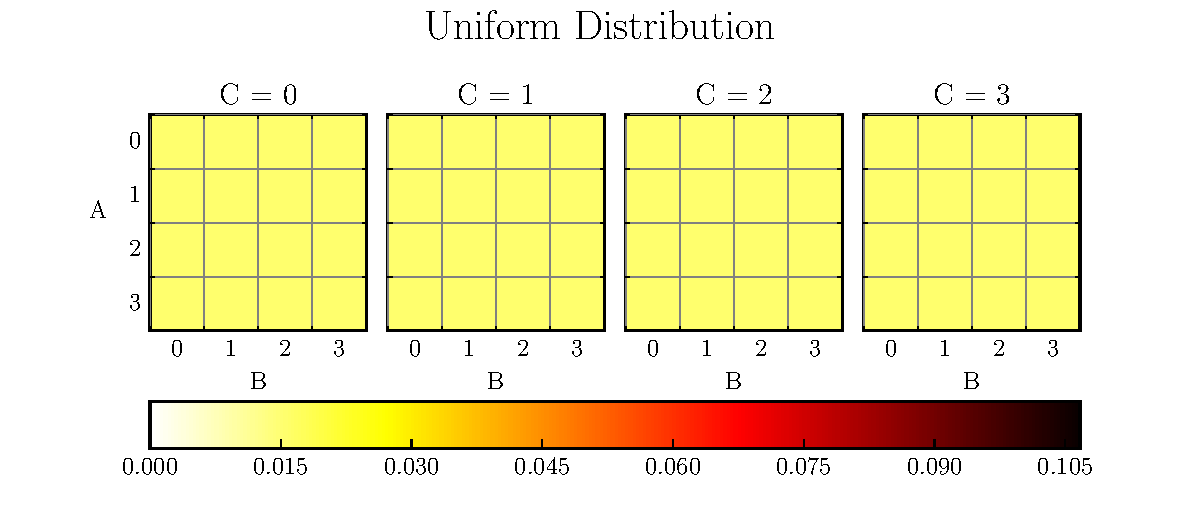
\includegraphics[scale=0.6,trim={0 0 0 0.4in},clip]{../../figures/distributions/uniform_dist_plot.pdf}
            \vspace{-0.2in}
            \[ \probplotvalue{255, 255, 109} = \f{1}{64} \]
            \caption{The completely uniform distribution $\s{U}$ visualized using a $4 \times 4 \times 4$ grid.}
            \label{fig:uniform_distribution}
    \end{center}
    \end{figure}
    In his original work, \citet{Fritz_2012} was able to find quantum non-classicality in the triangle scenario by embedding Bell non-classicality. As was mentioned in \cref{sec:fritz_distribution}, this embedding required a very idealistic condition to hold: perfect correlations between $C$ and $A_l, B_l$. From an experimental point of view, it is impossible to use Fritz's original argument to confirm non-classicality because every observable distribution is subject to \text{noise}. It is possible to minimize noise by developing more accurate measurement channels but perfect correlations are too idealistic. Causal compatibility inequalities not only permit there to be noise within a set of observations, but they also provide a means of quantifying the amount of noise that is allowed before non-classicality breaks down. \\

    In the triangle scenario, we define a completely noisy observation as the uniform probability distribution $\s{U} = \s{U}_{ABC}$ (see \cref{fig:uniform_distribution})
    \[ \s{U}\br{abc} = \s{U}_{ABC}\br{abc} = \f{1}{64} \quad \forall a,b,c\in \bc{0,1,2,3}  \]
    Since the uniform distribution $\s{U}$ is trivially compatible with the triangle scenario, the objective of this section is to determine how much uniform noise needs to be added to the Fritz distribution $\prob[\fritz]$ before it transitions from incompatible to compatible. We do this by defining an affine noise parameter $\vep$ such that $0 \leq \vep \leq 1$ along with the \term{noisy variant} $\s{N}_{\vep}$ of the Fritz distribution,
    \[ \s{N}_{\vep} = \br{1 - \vep} \prob[\fritz] + \vep \s{U} \]
    Therefore as $\vep$ varies from $0$ to $1$, more and more noise is added to the Fritz distribution as $\s{N}_{\vep}$ transitions from an incompatible distribution $\s{N}_{0} = \prob[\fritz]$ to a compatible distribution $\s{N}_{1} = \s{U}$. For each inequality $I$ and distribution $\prob$, let $I\br{\prob}$ denote a scalar value representing the amount of violation seen by $\prob$. As a standard, let $I\br{\prob} < 0$ represent violations while $I\br{\prob} \leq 0$ represents satisfaction of $I$ (with $I\br{\prob} = 0$ corresponding to complete saturations of the inequality). \\

    To analyze noise, $4$ inequalities where chosen. First, $I_0$ is the inequality derived using the Wagon-Wheel wheel inflation \cref{eq:ww_ineq}. The other three inequalities $I_1, I_2, I_3$ were all derived using the Web inflation; $I_1$ can be found in \cref{sec:web_inequality} while $I_3$ is the symmetric inequality in \cref{sec:symmetic_web_inequality}. Inequality $I_2$ is not reproduced anywhere in this document but is similar to \cref{sec:web_inequality}.

    \begin{center}
    \begin{figure}
    \begin{subfigure}[b]{.48\linewidth}
    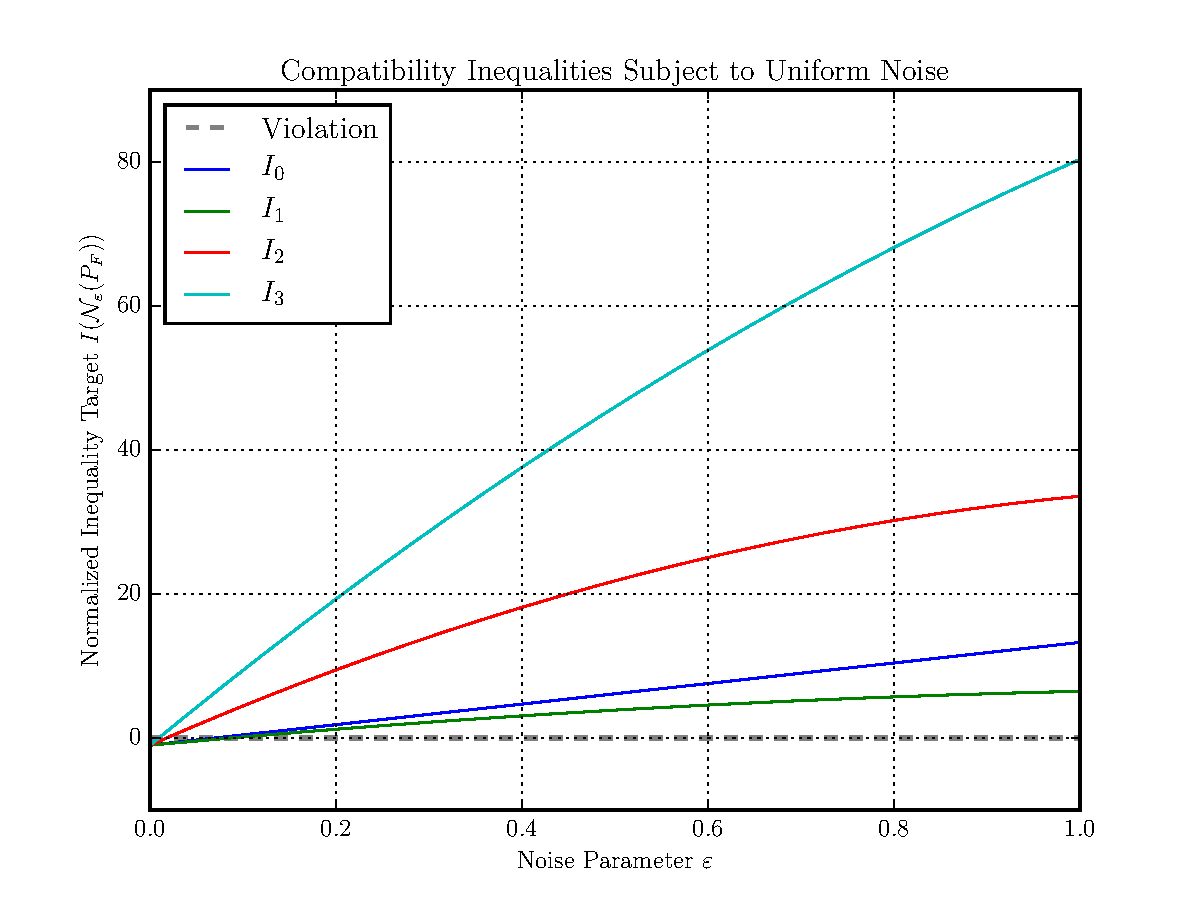
\includegraphics[width=\linewidth]{../../figures/noise/noise_2017.pdf}
    \caption{Complete range of noise parameters $\vep$.}\label{fig:noise}
    \end{subfigure}
    \begin{subfigure}[b]{.48\linewidth}
    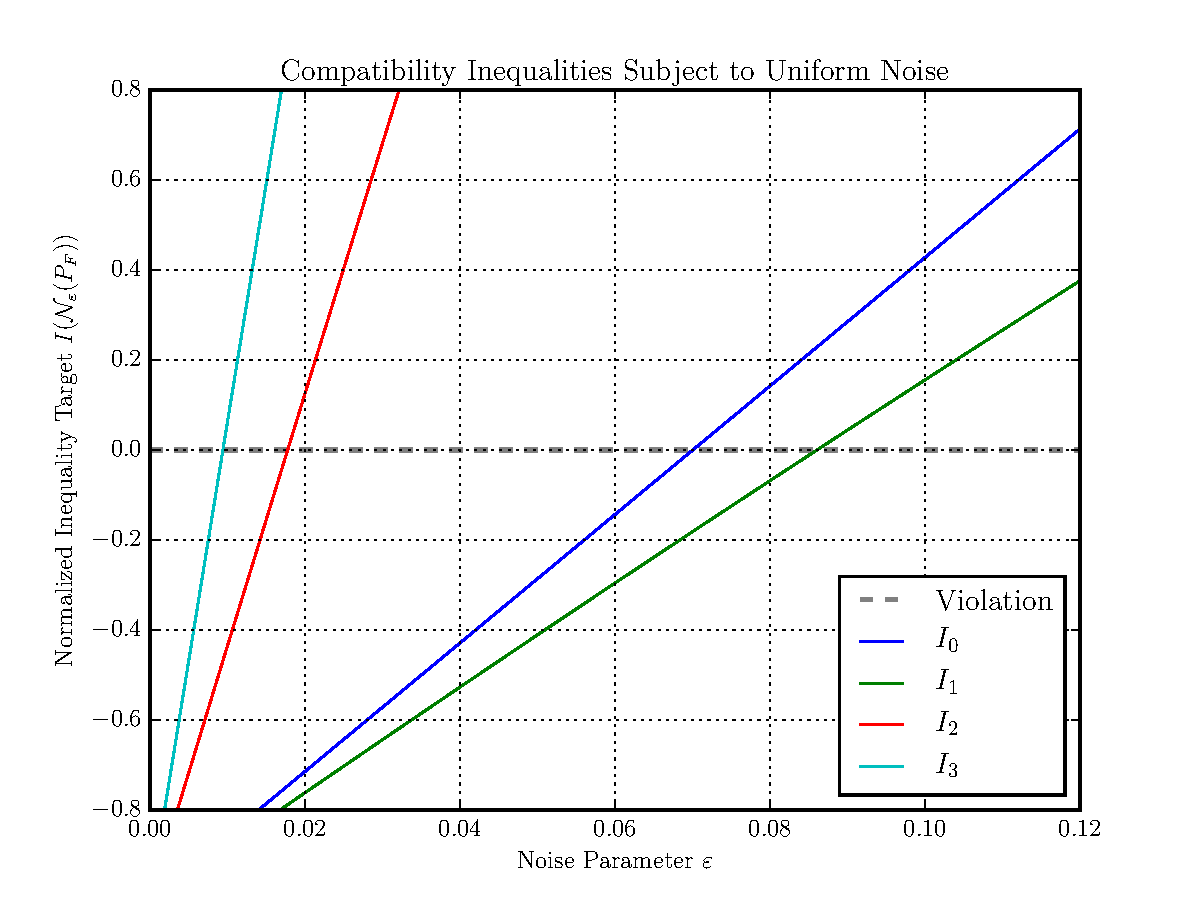
\includegraphics[width=\linewidth]{../../figures/noise/noise_2017_lims.pdf}
    \caption{\Cref{fig:noise} zoomed onto relevant region.}\label{fig:noise_zoomed}
    \end{subfigure}
    \caption{Inequality violations when subjected to uniform noise. Each inequality is normalized so that maximum violation is $-1$.}\label{fig:master_noise}
    \end{figure}
    \end{center}

    The results of our experiments are plotted in \cref{fig:master_noise}. \Cref{fig:noise} illustrates that each curve $I\br{\s{N}_{\vep}\br{\prob[\fritz]}}$ as a function of $\vep$ is monotonically increasing as expected; the more noise added to the probability distribution, the more classical it becomes. \Cref{fig:noise_zoomed} is the same plot as \cref{fig:noise} zoomed onto the interval $\vep \in \bs{0, 0.12}$. These tests suggest that inequality $I_1$ (\cref{sec:web_inequality}), when compared against all others is most robust to noise. \\

    Overall, this noise model demonstrates that the Fritz distribution remains incompatible with the triangle scenario up to at least a noise parameter of $\vep \simeq 0.085$. The associated distribution $\s N_{0.085}\br{\prob[\fritz]}$ is plotted in \cref{fig:noisy_fritz}. There remains the possibility that another inequality will be able to withstand a larger degree of noise that $I_1$. Given that $I_0, I_1, I_2, I_3$ are far from a representative inequalities and are likely not facets of any inflated marginal polytope, it is save to say that this is possible.

    \begin{figure}
    \begin{center}
            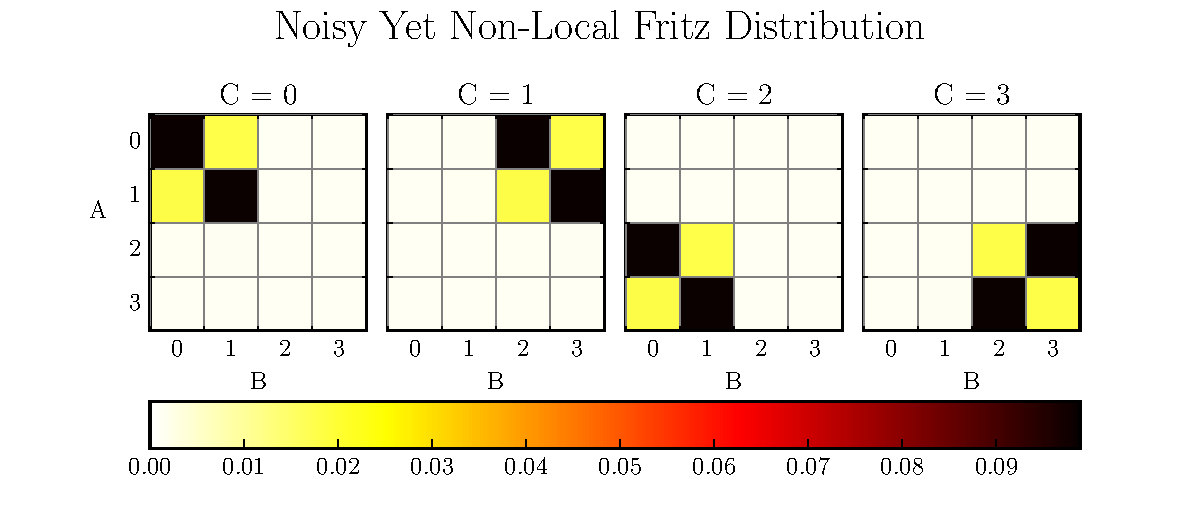
\includegraphics[scale=0.6,trim={0 0 0 0.4in},clip]{../../figures/noise/noisy_yet_non_local_fritz.pdf}
            \vspace{-0.2in}
            \[ \probplotvalue{255, 255, 243} = 0.00133 \]
            \caption{$\s{N}_{0.085}$: A noisy yet still non-classical variant of the Fritz distribution.}
            \label{fig:noisy_fritz}
    \end{center}
    \end{figure}

    \subsection{Numerical Optimizations}
    \label{sec:optimizations}
    Causal compatibility inequalities act as a \textit{measure} of non-classicality. If two non-classical distributions $\prob[1]$ and $\prob[2]$ violate the same inequality $I$ with violations $I\br{\prob[1]}$ and $I\br{\prob[2]}$ respectively, it is somewhat reasonable to say that $\prob[1]$ is \textit{more} non-classical than $\prob[2]$ whenever ${I\br{\prob[1]}} < I\br{\prob[2]}$\footnote{Remember that larger violations are more negative when the inequalities are written in the proposed canonical form.} Nonetheless, this statement comes from several caveats. First, it is possible (and frequently the case) for ${I\br{\prob[1]}} < I\br{\prob[2]}$ to hold for one inequality $I$ but have ${\ti I\br{\prob[2]}} < \ti I\br{\prob[1]}$ hold for another inequality $\ti I$. In this case, all one can claim is that $\prob[1]$ is more incompatible than $\prob[2]$ with respective to $I$ but the contrary is true with respect to $\ti I$. Second, not all inequalities $I$ are \textit{good} measures of non-classicality. In the case of the Bell scenario, the linear inequality constraints associated with the facets of the marginal polytope are the best measures of non-classicality. This is because the facets form a necessary and sufficient set with all other inequalities following from positive mixtures of the facets. However, good measures of incompatibility are less understood in the triangle scenario where the space of classical correlations is non-convex. At the very least, the inequalities derived in this report are likely \textit{not} the best measures of incompatibility (especially because they are curated toward the Fritz distribution). Nonetheless, these inequalities act the \textit{first} measures of non-classicality in the triangle scenario.\\

    In order to find quantum distributions that are more non-classical than the Fritz, we performed numerical optimizations against a objective scalar function $f: \R^n \in \R$ using the following pipeline: To begin, a set of real-valued parameters $\la = \br{\la_0, \ldots, \la_n} \in \R^{n}$ are used to parameterize a set of quantum states $\rho_{AB}, \rho_{BC}, \rho_{CA}$ and measurements $M_A, M_B, M_C$ in agreement with the quantum version of the triangle scenario in \cref{fig:triangle_scenario_quantum_model}. Second, a $4$-outcome distribution $\prob[ABC]$ is obtained via \cref{eq:quantum_model_triangle} and supplanted into an inequality $I$ in homogeneous and canonical form $I\br{\prob[ABC]} \leq 0$. The objective value is simply the degree of violation $f = I\br{\prob[ABC]}$ and used to make adjustments to $\la$ in order to achieve largest and larger violations. \\

    Finding larger violations to compatibility inequalities is nothing more that a numerical optimization (specifically minimization) of $f\br{\la}$. Since the inequalities themselves are polynomial and the space of quantum-accessible distributions is non-convex, a number of optimization methods were used in an attempt to eliminate any issues associated with local minima or ill-conditioned convergence. Specifically, the BFGS method~\cite[p. 142]{Nocedal_2000} and the Nelder-Mead simplex method~\cite[p. 238]{Nocedal_2000} were used along with a hybrid method called Basin Hopping~\cite{Wales_1997}.

    \subsection{Parameterizing Quantum Distributions}
    \label{sec:param_quantum_dist}
    \begin{figure}
    \begin{center}
            \scalebox{1.0}{\begin{tikzpicture}[scale=1]
    \begin{scope}[every node/.style=observed]
        \node (C) at (-2, 0) {$M_C$};
        \node (B) at (2, 0) {$M_B$};
        \node (A) at (0, {2*sqrt(3)}) {$M_A$};
    \end{scope}
    \begin{scope}[every node/.style=latent]
        \node (X) at (-1, {sqrt(3)}) {$\rho_{CA}$};
        \node (Y) at (1, {sqrt(3)}) {$\rho_{AB}$};
        \node (Z) at (0, 0) {$\rho_{BC}$};
    \end{scope}
    \begin{scope}[every path/.style={draw=cause, thick}]
        \path[postaction={on each segment={mid arrow}}]
        (X) -- (A)
        (X) -- (C)
        (Y) -- (A)
        (Y) -- (B)
        (Z) -- (B)
        (Z) -- (C);
    \end{scope}
\end{tikzpicture}}
            \caption{The triangle scenario as modeled by quantum states and measurements.}
            \label{fig:triangle_scenario_quantum_model}
    \end{center}
    \end{figure}
    In search of new, incompatible, quantum distributions that can be realized on the triangle scenario, numerical optimizations over the the space of quantum-accessible probability distributions are performed. To do so, we are interested in a parameterization all distributions that can be expressed as follows:
    \[ \prob[\p{ABC}]\br{abc} = \Tr\bs{\netperm^\intercal \rho_{\p{AB}}\otimes\rho_{\p{BC}}\otimes\rho_{\p{CA}} \netperm M_{\p{A},a}\otimes M_{\p{B},b} \otimes M_{\p{C},c}} \eq \label{eq:quantum_model_triangle}\]
    Where $\rho_{\p{AB}}, \rho_{\p{BC}}, \rho_{\p{CA}}$ are bipartite density matrices, $M_{\p{A}}, M_{\p{B}}, M_{\p{C}}$ are generic measurements sets and $\netperm$ is a permutation matrix that aligns the states and measurements appropriately\footnote{$\netperm$ is discussed more thoroughly in \cref{sec:perm_matrix}.}. \\

    In order to qualify the scope of \cref{eq:quantum_model_triangle} and associated computational complexity of the parameterization, there are a two restrictions that are made with justification. The states $\rho$ are taken to be bipartite \textit{qubit} states acting on $\s{H}^{2} \otimes \s{H}^{2}$. This is motivated by \cref{sec:fritz_distribution} in which the Fritz distribution only requires qubit states. In generality, one could consider $n$-dimensional states acting on $\s{H}^{n} \otimes \s{H}^{n}$. However, in such cases the joint density matrix $\rho_{\p{AB}}\otimes\rho_{\p{BC}}\otimes\rho_{\p{CA}}$ then acts on $\br{\Hilb^{n}}^{\otimes 6}$ requiring a $n^6 \times n^6$ matrix with $n^{12}$ entries. Therefore, $n = 2$ is far more computationally feasible than $n > 2$. Additionally, restrict our focus to projective-valued measures (PVMs) instead of projective-operator valued measures (POVMs) for three reasons. First, \cref{sec:fritz_distribution} demonstrates that PVMs are sufficient for witnessing incompatible quantum distributions in the triangle scenario. Second, generating $k$-outcome POVM measurements is possible using rejection sampling techniques~\cite{Petz_2015}, however a valid, unbiased parameterization was not found for $k > 2$. Finally, PVMs provide considerable computational advantage over POVMs as they permit \cref{eq:quantum_model_triangle} to be re-written as follows:
    \[ \prob[\p{ABC}]\br{abc} = \bramidket{m_{\p{A},a}m_{\p{B},b}m_{\p{C},c}}{\netperm^\intercal \rho_{AB}\otimes\rho_{BC}\otimes\rho_{CA} \netperm}{m_{\p{A},a}m_{\p{B},b}m_{\p{C},c}} \eq \label{eq:quantum_model_triangle_pvms}\]

    In order to parameterize all such distributions, we elect to parameterize the states and measurements separately. Although there are numerous techniques that can used when parameterizing quantum states and measurements~\cite{Petz_2015, Hedemann_2013,Fujii_2005,James_2001,Grasmair_2014,Neilsen_Chaung_2011}, a single technique is presented that was found to be most computationally suitable for our purposes.
    \subsubsection{Unitary Group}
    \label{sec:unitary_group}
    To facilitate the parameterization of quantum states states and PVMs, a parameterization of the unitary group of dimension $d$ (denoted $\s{U}\br{d}$) by Spengler, Huber and Hiesmayr~\cite{Spengler_2010_Unitary} is introduced. Discussions of its application to states and measurements are deferred to \cref{sec:states} and \cref{sec:measurements} respectively.

    In Ref.~\cite{Spengler_2010_Unitary}, Spengler \textit{et al.} proved that all unitaries $U \in \s{U}\br{d}$ can be parameterized without degeneracy as follows:
    \[ U = \bs{\prod_{m=1}^{d-1} \br{\prod_{n=m+1}^{d} \exp\br{i P_n \lambda_{n,m}}\exp\br{i \si_{m,n} \lambda_{m,n}}}} \tcdot \bs{\prod_{l=1}^{d} \exp\br{iP_l \lambda_{l,l}}}  \eq \label{eq:spengler_unitary} \]
    Where $\la = \bc{\la_{n,m} \mid n,m \in 1, \ldots, d}$ form a $d \times d$ matrix of real-valued parameters with periodicities $\la_{m,n} \in \bs{0, \f{\pi}{2}}$ for $m < n$ and $\la_{m,n} \in \bs{0, 2 \pi}$ for $m \geq n$.
    \[ \la = \begin{pmatrix}
        \la_{1,1} & \cdots & \la_{1, d} \\
        \vdots & \ddots & \vdots \\
        \la_{d,1} & \cdots & \la_{d, d} \\
    \end{pmatrix} \]
    And where $P_l$ are one-dimensional projective operators,
    \[ P_l = \ket{l}\bra{l} \qquad 1 \leq l \leq d \eq \label{eq:projective_operator} \]
    and the $\si_{m,n}$ are generalized anti-symmetric $\si$-matrices,
    \[ \sigma_{m,n} = -i \ket{m}\bra{n} +i \ket{n}\bra{m} \qquad 1 \leq m < n \leq d\]
    The SSH parameterization (\cref{eq:spengler_unitary}) is unique in that each of the real-valued parameters $\la_{n,m}$ has physical significance. For the sake of reference, let us label the matrix exponential terms in \cref{eq:spengler_unitary} in a manner that corresponds to their affect on an orthonormal basis $\bc{\ket{1}, \ldots, \ket{d}}$.
    \begin{align*}
    \begin{split}
        GP_l &= \exp\br{iP_l \lambda_{l,l}} \\
        RP_{n,m} &= \exp\br{i P_n \lambda_{n,m}} \\
        R_{m,n} &= \exp\br{i \si_{m,n} \lambda_{m,n}}
    \end{split} \eq \label{eq:exp_terms}
    \end{align*}
    For example, $R_{m,n} = \exp\br{i \si_{m,n} \lambda_{m,n}}$ applies a rotation to the sub-space spanned by $\ket{m}$ and $\ket{n}$ for $m < n$. Analogously, $RP_{n,m}$ generates the relative phase between $\ket{m}$ and $\ket{n}$ for $m > n$ and $GP_l$ fixes the global phase of $\ket{l}$. Possessing a parameterization that maintains this physical interpretation is useful as it allows one to readily eliminate any degeneracies. For the purposes of quantum distributions such as \cref{eq:quantum_model_triangle}, it should be clear that any contributions to global phase are irrelevant. The SSH parameterization becomes especially attractive because it readily permits one to drop the global phase terms by setting $\la_{l,l} = 0$ for all $l = 1, \ldots, d$. It is convenient to denote the set of all unitaries up to global phase considerations as $\ti {\s{U}}\br{d}$ and express $\ti {U} \in \ti {\s{U}}\br{d}$ using $d\br{d-1}$ real-valued parameters:
    \[ \ti U = \prod_{m=1}^{d-1} \br{\prod_{n=m+1}^{d} RP_{n,m}R_{m,n}} \eq \label{eq:spengler_unitary_gp} \]
    Another attractive feature of the SSH parameterization not mentioned in~\cite{Spengler_2010_Unitary} is that \cref{eq:spengler_unitary}, and thus \cref{eq:spengler_unitary_gp}, can be implemented in a computationally efficient manner. This is discussed in \cref{sec:comp_spengler}.
    \subsubsection{Measurements}
    \label{sec:measurements}
    For each measurement set $M$ in \cref{eq:quantum_model_triangle}, we consider a $d$-element projective-valued measure (PVM) $M = \bc{M_1, \ldots, M_d}$ satisfying a number of familiar constraints:
    \begin{gather*}
    \forall \ket{\phi} \in \Hilb^d: \bra{\phi} M_i \ket{\phi} \geq 0 \qquad \sum_{i=1}^{d} M_i = \ident_{d} \\
    M_i = \ket{m_i}\bra{m_i} \qquad M_i M_j = \de_{ij} M_i
    \end{gather*}
    Therefore, parameterizing $M$ corresponds to parameterizing the set of all orthonormal basis $\bc{\ket{\psi_1}, \ldots, \ket{\psi_d}}$ of $\Hilb^d$.
    First note that any such basis can be transformed into the computational basis $\bc{\ket{1}, \ldots, \ket{d}}$ by a unitary denoted $U^{-1} \in \mathcal{U}\br{d}$.
    \[ \forall i : U^{-1} \ket{\psi_i} = \ket{i} \eq \label{eq:unitary_transform}\]
    With this observation, all that is required is to parameterize the set of all unitaries $U \in \mathcal{U}\br{d}$. Specifically, the projective property each $M_i \in M$ means that the global phase of $U$ is completely arbitrary; one only needs to consider parameterizing unitaries up to global phase using \cref{eq:spengler_unitary_gp}.
    \[ M = \bc{\ti U \ket{i} \bra{i} \ti U^{\dagger} \mid i \in \bc{1, \ldots, d}} \]
    For the purposes discussed in \cref{sec:param_quantum_dist}, only $d = 4$ outcome measurements are utilized and therefore requiring $4\br{4 - 1} = 12$ real-valued parameters. This method was inspired by the measurement seeding method for iterative optimization used by \citet{Pal_2010} .
    \subsubsection{States}
    \label{sec:states}

    Each state $\rho \in \br{\rho_{AB}, \rho_{BC}, \rho_{CA}}$ of \cref{eq:quantum_model_triangle} is modeled as a two-qubit density matrices acting on $\Hilb^2 \otimes \Hilb^2$. The space of all such states corresponds to the space of all $4\times 4$ positive semi-definite hermitian matrices with unitary trace.
    \[ \forall \ket{\phi} \in \Hilb^d: \bra{\phi} \rho \ket{\phi} \geq 0 \qquad \rho^{\dagger} = \rho \qquad \Tr\br{\rho} = 1 \eq \label{eq:density_matrix}\]
    Although is common to parameterize all such matrices using a Cholesky decomposition~\cite{Grasmair_2014}, we make use of the non-degenerate SHH parameterization~\cite{Spengler_2010_Unitary} and the spectral decomposition of $\rho$. Retaining full generality, consider full-rank density matrices:
    \[ \rho = \sum_{i=1}^{d} p_i \ket{\psi_i}\bra{\psi_i} \qquad \sum_{i=1}^{d} p_i = 1, p_i \geq 0 \eq \label{eq:param_density} \]
    Where $\bc{p_i}$ are the eigenvalues of $\rho$ and $\bc{\ket{\psi_i}}$ are its eigenstates. It is here that one recognizes the reapplication of \cref{eq:unitary_transform}: any orthonormal basis $\bc{\ket{\psi_i}}$ of $\Hilb^d$ can be transformed into a computational basis $\bc{\ket{i}}$ by a unitary transformation $U \in \mathcal{U}\br{d}$ such that $\ket{\psi_i} = U\ket{i}$. Analogous to the projective measurements considered in \cref{sec:measurements}, the global phase contributions are redundant.
    \[ \rho = \sum_{i=1}^{d} p_i \ti U\ket{i}\bra{i} \ti U^{\dagger} \]
    Parameterizing the eigenvalues requires $d - 1$ real-valued parameters due to the trace constraint of \cref{eq:density_matrix}. The eigenvalues are parameterized without degeneracy using a tuple of $d-1$ parameters $\lambda = \br{\lambda_1, \ldots, \lambda_{d-1}}, \lambda_i \in \bs{0, 2 \pi}$ using hyper-spherical coordinates~\cite{Hedemann_2013, Spengler_2010_Unitary}:
    \begin{align*}
    \eq \label{eq:convex_param}
    \begin{split}
        p_n &= \prod_{i=1}^{n-1} \sin^2 \lambda_i \\
        p_j &= \cos^2 \lambda_j \prod_{i=1}^{j-1} \sin^2 \lambda_i \quad \forall j \in 1, \ldots, n - 1
    \end{split}
    \end{align*}

    Furthermore due to the periodicity of the parameter space $\bc{\lambda}$, \cref{eq:convex_param} can be used for either constrained or unconstrained optimization problems. For continuity reasons, unconstrained optimizations are performed whenever possible. In conclusion, it is possible to parametrize all $d$-dimensional density matrices satisfying \cref{eq:density_matrix} using $d\br{d - 1} + d - 1 = d^2 -1$ real-valued parameters. \\

    Although non-degenerate, \cref{eq:convex_param} suffers from a lack of uniformity; a randomly sampled vector of parameters $\bc{\lambda}$ \textit{does not} translate to a randomly sampled set of eigenvalues $\bc{p_i}$. Another, albeit degenerate, parameterization of $\bc{p_i}$ involves beginning with $d$ real parameters $\lambda = \br{\lambda_1, \ldots, \lambda_d}$, then forcing normalization by dividing each parameter $\la_i$ by the their sum.\footnote{Strictly speaking, \cref{eq:uniform_param} \textit{also} suffers from non-uniformity; being biased toward eigenvalues that have similar values to each other.}.
    \[ p_j = \f{\abs{\lambda_j}}{\sum_{i=1}^{n} \abs{\lambda_i}} \quad \forall j \in 1, \ldots, n \eq \label{eq:uniform_param} \]
    For various optimization tasks sensitive to initial conditions outlined \cref{sec:optimizations}, the latter parameterization of \cref{eq:uniform_param} generally performed better than the former \cref{eq:convex_param}.
    \subsubsection{Permutation Matrix}
    \label{sec:perm_matrix}
    \begin{figure}
        \centering
        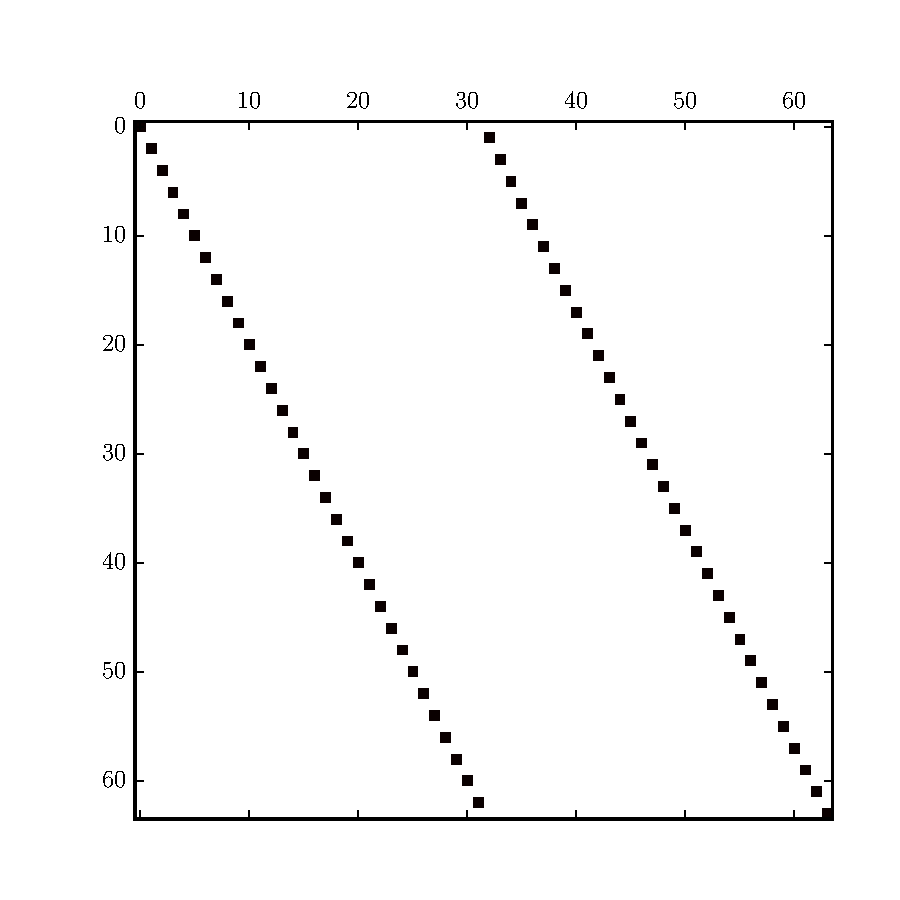
\includegraphics[trim={1cm 1.2cm 1.0cm 1cm},clip,width=0.4\textwidth]{../../figures/perm_mtrx.pdf}
        \caption{The permutation matrix $\netperm$ acting on $\br{\Hilb^2}^{\otimes 6}$ for the triangle scenario. Black entries represents a value of $1$ and white represents $0$.}
        \label{fig:perm_mtrx}
    \end{figure}
    Finally, we introduce the a permutation matrix $\netperm$ for the triangle scenario. For bipartite qubit states, $\netperm$ is the $64\times64$ bit-wise matrix depicted in \cref{fig:perm_mtrx}. Upon examination of \cref{eq:quantum_model_triangle_pvms}, we consider $\netperm$ to be acting on the joint global state $\rho_{\p{AB}} \otimes \rho_{\p{BC}} \otimes \rho_{\p{CA}}$. To illuminate its necessity, consider \cref{eq:quantum_model_triangle} in the absence of $\netperm$.
    \begin{align*}
    \prob[\p{ABC}]\br{abc} &\stackrel{?}{=} \Tr\bs{\br{\rho_{\p{AB}} \otimes \rho_{\p{BC}} \otimes \rho_{\p{CA}}} \br{M^a_{\p{A}}\otimes M^b_{\p{B}} \otimes M^c_{\p{C}}}}\\
    &= \Tr\bs{\br{\rho_{\p{AB}}M^a_{\p{A}}}\otimes\br{\rho_{\p{BC}}M^b_{\p{B}}}\otimes\br{\rho_{\p{CA}}M^c_{\p{C}}}}\\
    &= \Tr\br{\rho_{\p{AB}}M^a_{\p{A}}}\Tr\br{\rho_{\p{BC}}M^b_{\p{B}}}\Tr\br{\rho_{\p{CA}}M^c_{\p{C}}}\\
    &= \prob[\p{A}\mid \rho_{\p{AB}}]\br{a}\prob[\p{B}\mid \rho_{\p{BC}}]\br{b}\prob[\p{C}\mid \rho_{\p{CA}}]\br{c}
    \end{align*}
    On an operational level, this corresponds to $A$ making a measurement on \textit{both} subsystems of $\rho_{AB}$ and \textit{not} on any component of $\rho_{CA}$. This is analogously troubling for $B$ and $C$ as well. To resolve this issue, the permutation matrix $\netperm$ corresponds to \textit{aligning} the underlying $6$-qubit joint state $\rho$ with the joint measurement $M$. To understand its effect, consider its effect on $6$-qubit pure state $\ket{q_1} \otimes \cdots \otimes \ket{q_6} = \ket{q_1q_2q_3q_4q_5q_6}$ where $\forall i : \ket{q_i} \in \Hilb^2$.
    \[ \netperm\ket{q_1q_2q_3q_4q_5q_6} = \ket{q_2q_3q_4q_5q_6q_1} \]
    $\netperm$ acts as a \textit{partial transpose} on $\br{\Hilb^2}^{\otimes 6}$ by shifting the underlying tensor structure one subsystem to the ``left''. It is uniquely defined by its action on all $2^6$ orthonormal basis elements of $\br{\Hilb^2}^{\otimes 6}$,
    \[ \netperm \defined \sum_{\ket{q_i} \in \bc{\ket{0}, \ket{1}}}\ket{q_2q_3q_4q_5q_6q_1}\bra{q_1q_2q_3q_4q_5q_6} \]
    \subsection{Numerical Optimization Results}
    \label{sec:results}

    \Cref{sec:param_quantum_dist} expounded on how we elected to parameterized the space of quantum distributions that can be realized on the quantum triangle scenario (\cref{fig:triangle_scenario_quantum_model}). Specifically, we make use of fully generic $4\times 4$ density matrices (bipartite qubit) for each shared resource and $4$-element projective measurements. For each inequality $I$, we define the relative violation $V_F$ to be maximum violation relative to the violation achieved by the Fritz distribution.
    \[ V_F = \f{\min_{P}\bc{I\br{P}}}{I\br{P_F}} \]

    The first inequality in consideration is $I_1$; the non-symmetric Web inflation inequality presented in \cref{sec:web_inequality}. At best, numerical optimizations converged to a distribution (\cref{fig:maximum_violation_I_1}) with relative violation $V_F \simeq 1.501$. Almost immediately, it is evident that \cref{fig:maximum_violation_I_1} closely resembles the Fritz distribution. In fact, \cref{fig:maximum_violation_I_1} and \cref{fig:fritz_distribution_visualized} share the exact same \textit{possibilistic structure} or set of possible events. What does this reveal about $I_1$ and non-classicality in the triangle scenario? This result is not entirely unexpected. As was mentioned in \cref{sec:found_inequalities}, these inequalities are derived specifically to show incompatibility of the triangle scenario. Consequently, it seems that $I_1$ only has the capacity to demonstrate incompatibility for a specific forms of non-classicality that resemble the Fritz distribution very closely. \\

    \begin{figure}
    \begin{center}
            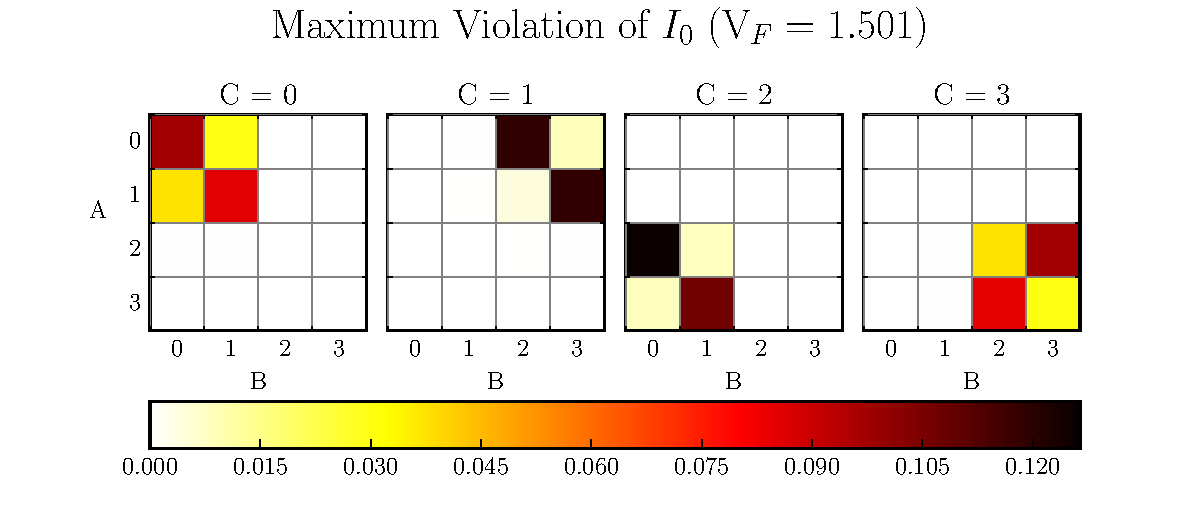
\includegraphics[scale=0.6,trim={0 0 0 0.4in},clip]{../../figures/distributions/plotted_dist_I_1_max_violation_2017.pdf}
            \caption{Probability distribution that maximizes violation of $I_1$ from \cref{sec:web_inequality} ($V_F \simeq 1.501$).}
            \label{fig:maximum_violation_I_1}
    \end{center}
    \end{figure}

    An alternative explanation has to do with the sensitively of the initial condition $\la_{\br{0}} = \br{\la_{\br{0}, 0}, \ldots, \la_{\br{0}, n}}$ in our optimization. In \cref{sec:param_quantum_dist}, it was shown that our parameter space of choice was $2\pi$-periodic in all entries. Somewhat surprisingly, when using a uniform seed for $\la_0$, all optimization methods consistently converged to inequality saturation instead of inequality violation which of course is achievable by the Fritz distribution. Instead, only initial seeds close enough to the \textit{Fritz parameters} $\la_{\br{\fritz}}$ (the parameters that induce the Fritz distribution using the quantum implementation in \cref{sec:fritz_distribution}) where able to achieve violation. To illustrate this graphically, we let the initial seed be a small Gaussian perturbation $\de \la$ away from $\la_{\br{\fritz}}$ in parameter space.
    \[ \la_{\br{0}} = \la_{\br{\fritz}} + \de \la  \]
    The Gaussian perturbation was given zero mean $\mu = 0$ and variance $\si^2 = \br{2 \pi 10^{\chi}}^2$ where $\chi$ measures an order of magnitude standard deviation. For $I_1$, deviations of $\chi \gtrsim 1.3$ inhibited convergence to violation. This is depicted in \cref{fig:initial_conditions}. Therefore, it is unclear whether or not our results share the same possibilistic structure as $\prob[\fritz]$ because of the inequality itself or the ill-conditioned nature of the optimization. Most likely, this phenomena is due to a combination of both effects.
    \begin{center}
    \begin{figure}
    \begin{subfigure}[t]{.48\linewidth}
    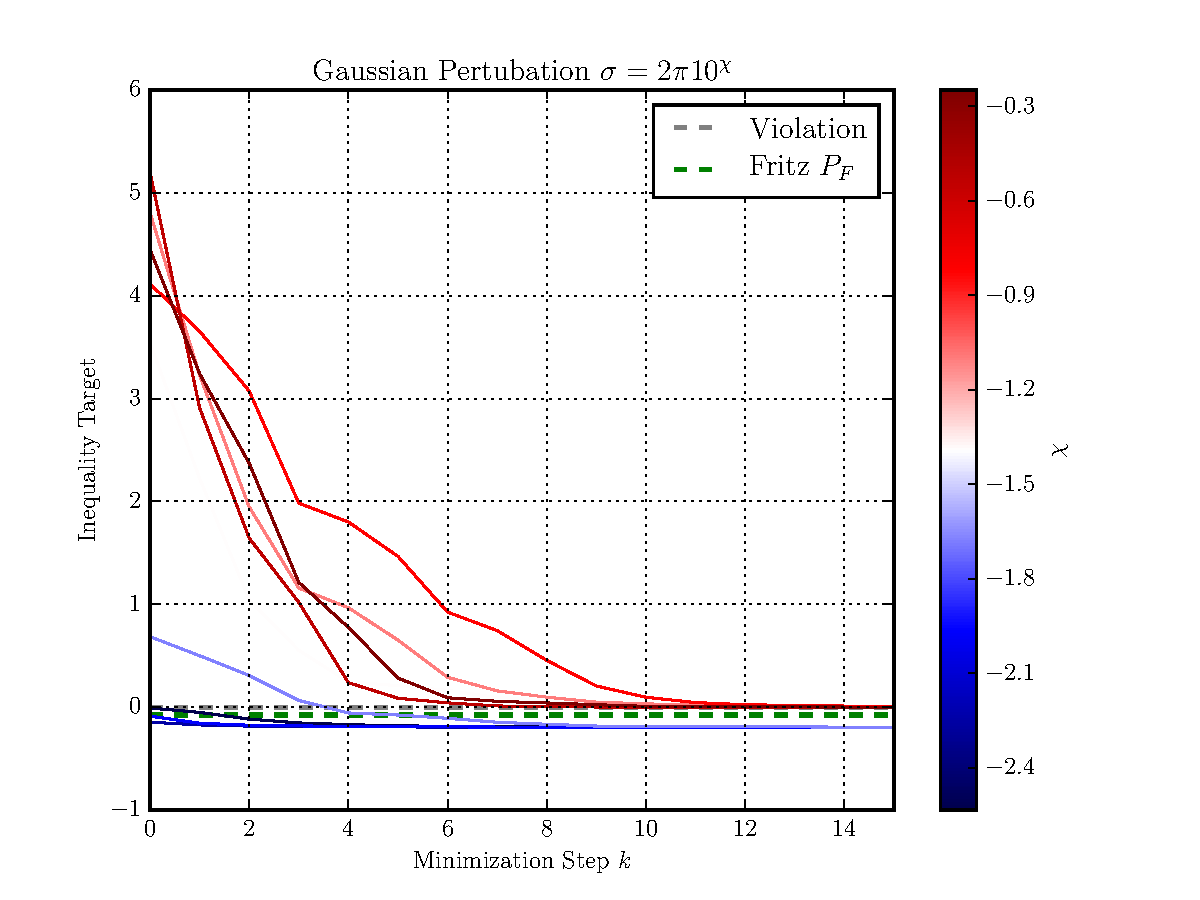
\includegraphics[width=\linewidth]{../../figures/optimizations/Gaussian_Perturbation_Fritz_Color_Default.pdf}
    \caption{For each iteration step $k$, the inequality target decreases.}\label{fig:initial_conditions_a}
    \end{subfigure}
    \begin{subfigure}[t]{.48\linewidth}
    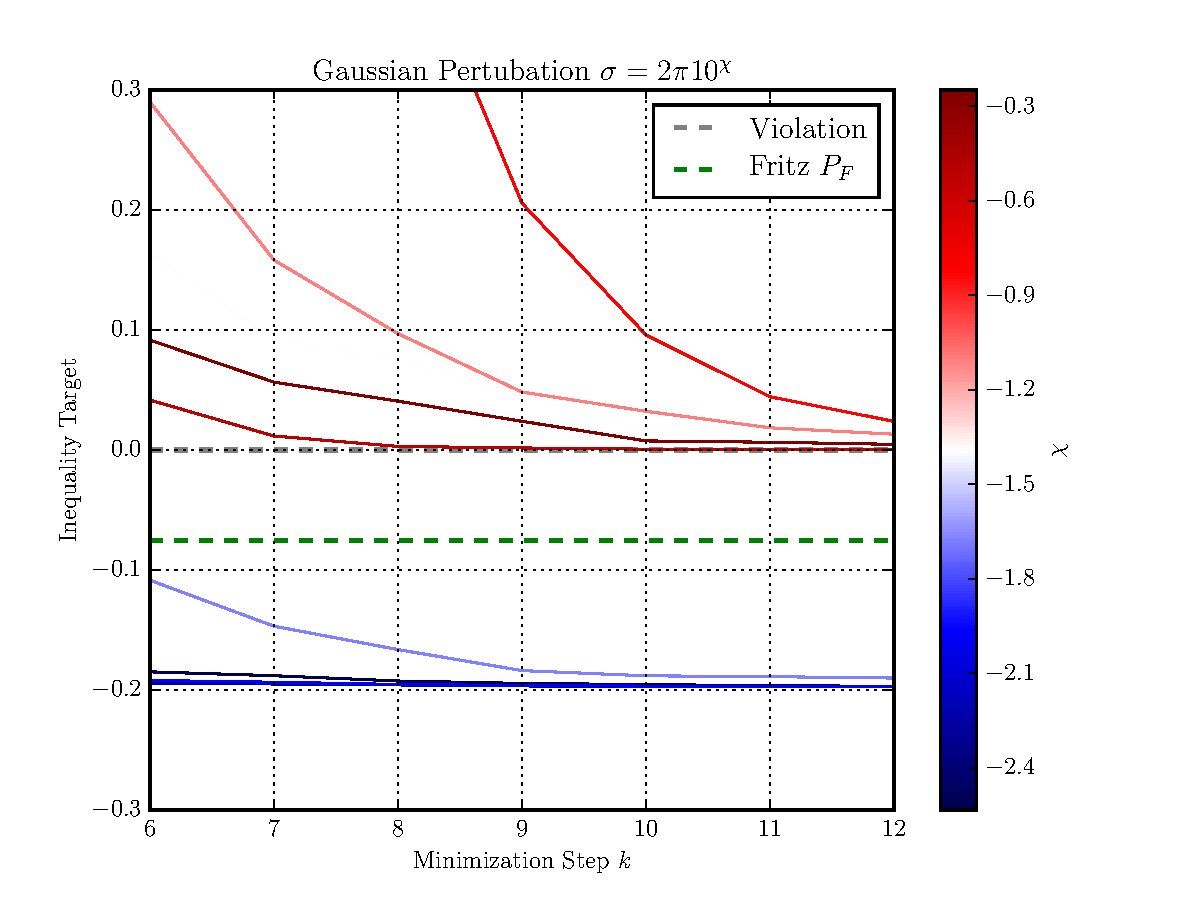
\includegraphics[width=\linewidth]{../../figures/optimizations/Gaussian_Perturbation_Fritz_Color_Zoomed.pdf}
    \caption{\Cref{fig:noise} zoomed to show convergence is sensitive to initial conditions.}\label{fig:initial_conditions_b}
    \end{subfigure}
    \caption{Numerical optimizations aimed at violating causal compatibility inequalities are sensitive to initial conditions.}\label{fig:initial_conditions}
    \end{figure}
    \end{center}
    The second inequality in consideration is $I_3$; the \textit{symmetric} Web inflation inequality presented in \cref{sec:symmetic_web_inequality}. This inequality was able to achieve a greater relative violation than $I_1$ as optimizations converged to a distribution (\cref{fig:maximum_violation_I_3}) with relative violation $V_F \simeq 2.61$. Just as before, the maximum violating distribution shares a possibilistic structure with the Fritz distribution. However, this result is far more surprising. Since the inequality is symmetric with respect to the exchange of parties $\varphi \in \Perm{A, B, C}$, one would naively expect that the maximum violating distribution is be symmetric as well. If it were not, one could construct a distribution that violates $I_3$ more by symmetrizing $\prob[\fritz]$ by summing over all possible permutations and normalizing. The symmetrized Fritz distribution is plotted in \cref{fig:symmetrized_fritz}. This distribution is also non-classical with relative violation $V_F = 3$. As it turns out, the symmetrized Fritz distribution is \textit{not} quantum-accessible in the sense that is cannot be written as \cref{eq:quantum_model_triangle}\footnote{At least numerical optimizations suggest this is the case.} Therefore we conclude that the space of quantum accessible correlations on the triangle scenario is non-convex; a reiteration of a result found in~\citet{Inflation}.
    \begin{figure}
    \begin{center}
            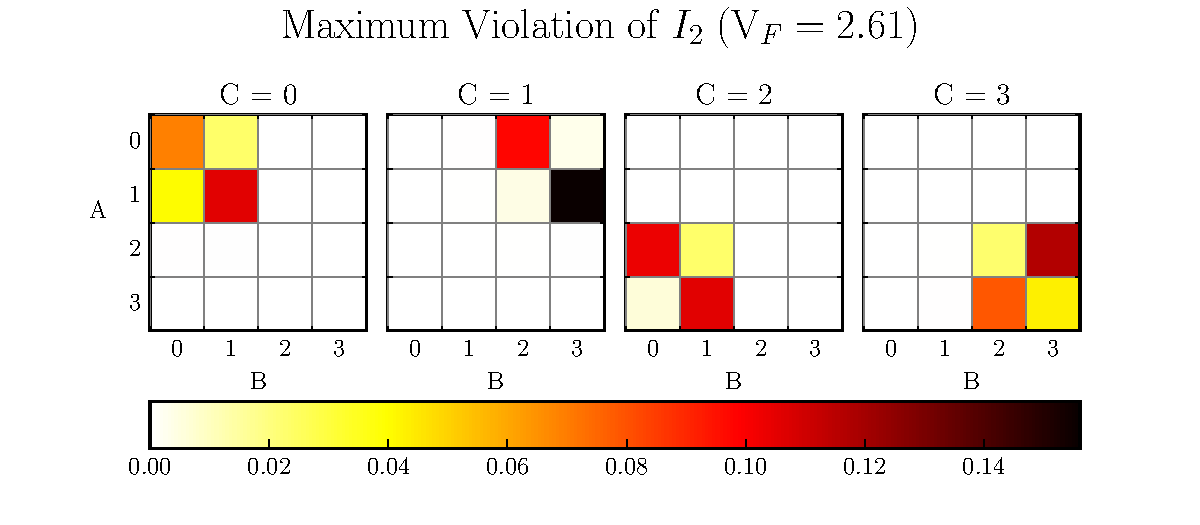
\includegraphics[scale=0.6,trim={0 0 0 0.4in},clip]{../../figures/distributions/plotted_dist_I_3_max_violation_2017.pdf}
            \caption{Probability distribution that maximizes violation of $I_3$ from \cref{sec:symmetic_web_inequality} ($V_F \simeq 2.61$).}
            \label{fig:maximum_violation_I_3}
    \end{center}
    \end{figure}
    \begin{figure}
    \begin{center}
            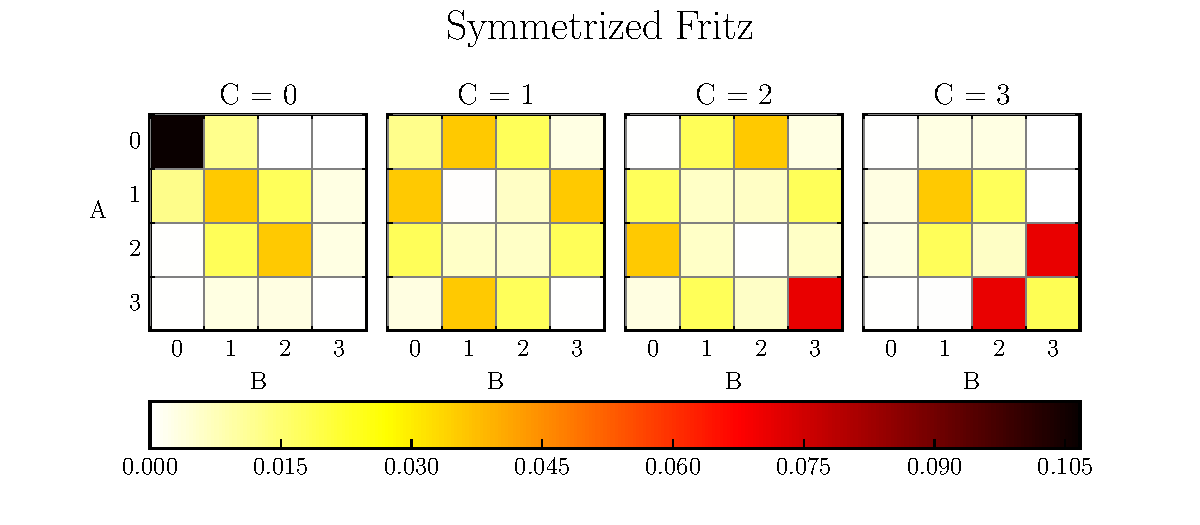
\includegraphics[scale=0.6,trim={0 0 0 0.4in},clip]{../../figures/distributions/symmetrized_fritz.pdf}
            \caption{Symmetrized version of the Fritz distribution ($V_F \simeq 3$).}
            \label{fig:symmetrized_fritz}
    \end{center}
    \end{figure}

    Finally for both $I_0$ and $I_2$, the maximum relative violation happens to be $V_F = 1$ (up to numerical precision). This means that the Fritz distribution either represents a local minimum of the parameter space or is in fact \textit{the} maximally violating distribution. Without further investigations, it is unclear if this behavior is related to the universality of the Fritz distribution or if its an artifact of the methods used to derive $I_0$ and $I_2$.

    \section{Conclusions}

    In \cref{sec:triangle_scenario}, we elucidated that non-classicality in the triangle scenario has been an unsolved problem for nearly a decade. Initially,~\citet{Branciard_2012} identified the triangle scenario as a challenging causal structure for studying non-classicality. Afterwards,~\citet{Henson_2014} were able to to classify the triangle scenario as \textit{interesting} which partially explains why it remains an enigma. Recently,~\citet{Fritz_2012} discovered the Fritz distribution as the first example of quantum non-classicality in the triangle scenario. Heretofore, researchers have been able to derive causal incompatibility inequalities~\cite{Inflation,Steudel_2010,Henson_2014} but unable to show that any are non-trivial in the context of quantum non-classicality. In \cref{sec:fritz_distribution} the Fritz distribution was introduced in detail and refinements where made to a problem originally proposed by~\citet{Fritz_2012}. For this research project, we made heavy use of the Inflation Technique of \cref{sec:inflation_technique} and the Fritz distribution in order to derive the first causal compatibility inequalities capable of having quantum violations. Finally, we used those inequalities in an attempt to discover new forms of non-classicality in the triangle scenario with partial success.\\

    Ultimately, this work accomplishes two important tasks. First and foremost, the derivation of \cref{eq:ww_ineq} demonstrates the utility of the Inflation technique specifically for quantum causal inference problems. The Inflation Technique was able to derive causal compatibility inequalities that admit quantum violations in the triangle scenario -- a task that no other existing techniques succeeded at. Therefore, this work acts as a strong indication that the Inflation technique has the potential to solve a assortment of unsolved causal inference problems including those manifest in quantum foundations and quantum information theory. \\

    Penultimately, the results presented here solve~\cite[Problem 2.17]{Fritz_2012} insofar as to refine the original problem into three related questions problems: \ref{r:1}, \ref{r:2} and \ref{r:3}. The methods and techniques demonstrated here provide a means of solving \ref{r:1} and gives an opportunity to begin tackling \ref{r:2} and \ref{r:3} in the form of numerical optimizations. Computational and comprehensive limitations have stunted progress towards solving \ref{r:2} and \ref{r:3}, so it still remains unclear if \ref{r:2} and \ref{r:3} have affirmative solutions in the first place.

    \section*{Acknowledgments}
    T.C. Fraser would like to thank E. Wolfe for his excellent guidance and mentor-ship throughout the duration of this research project. Moreover, T.C. Fraser would like to thank the Perimeter Institute for financing this research and providing access to much needed computational resources.
    \clearpage
    \bibliography{../references}

    \clearpage
    \appendix


    \section{Common Terminology \& Notation}

    \subsection{Graph Theory}
    \label{sec:graph_theory}
    \begin{definition}
        \label{def:graph}
        A \term{graph} $\graph$ is an ordered tuple $\br{\nodes, \edges}$ of \textit{nodes} and \textit{edges} respectively where the nodes have the capacity to represent any object while the edges are defined as \textit{pairs} of nodes $\edges \subseteq \nodes \times \nodes$. A \term{directed graph} $\graph$ is a graph where each edge $e \in \edges$ is assigned an order or \term{direction} $e = \bc{n \to n'}$.
    \end{definition}

    \begin{definition}
        \label{def:graph_terms}
        The following definitions are common language in directed graph theory. Let $n, m \in \nodes$ be example nodes of the graph $\graph$.
        \begin{itemize}
            \item The \term{parents of a node}: $\Pa[\graph]{n} \defined \bc{m \mid m \to n}$
            \item The \term{children of a node}: $\Ch[\graph]{n} \defined \bc{m \mid n \to m}$
            \item The \term{ancestry of a node}: $\An[\graph]{n} \defined \bigcup_{i\in\mathbb{W}} \Pa[\graph][i]{n}$ where $\Pa[\graph][i]{n} \defined \Pa[\graph]{\Pa[\graph][i-1]{n}}$ and $\Pa[\graph][0]{n} = n$
            \item The \term{descendants of a node}:  $\De[\graph]{n} \defined \bigcup_{i\in\mathbb{N}} \Ch[\graph][i]{n}$ where $\Ch[\graph][i]{n} \defined \Ch[\graph]{\Ch[\graph][i-1]{n}}$ and $\Ch[\graph][1]{n} = \Ch[\graph]{n}$
        \end{itemize}
        All of these terms can be generalized to sets of nodes $N \subseteq \nodes$ through union over the elements,
        \begin{itemize}
            \item The \term{parents of a node set}: $\Pa[\graph]{N} \defined \bigcup_{n\in N}\Pa[\graph]{n}$
            \item The \term{children of a node set}: $\Ch[\graph]{N} \defined \bigcup_{n\in N}\Ch[\graph]{n}$
            \item The \term{ancestry of a node set}: $\An[\graph]{N} \defined \bigcup_{n\in N}\An[\graph]{n}$
        \end{itemize}
    \end{definition}

    \begin{definition}
        An \term{induced subgraph} of $\graph$ for a subset of nodes $N \subseteq \nodes$ is another graph composed of nodes $N$ and all edges $e$ of the original graph that are contained in $N$.
        \[ \Sub[\graph]{N} \defined \br{N, \bc{e = \bc{n \to n'} \mid n, n' \in N, e \in \edges}} \]
        An \term{ancestral subgraph} of $\graph$ for a subset of nodes $N \subseteq \nodes$ is the induced subgraph due to the ancestry of $N$.
        \[ \AnSub[\graph]{N} \defined \Sub[\graph]{\An[\graph]{N}} \]
    \end{definition}

    \begin{definition}
        \label{def:dag}
        A \term{directed acyclic graph} or \term{DAG} $\graph = \br{\nodes, \edges}$ is an directed graph with the additional property that no node $n$ is in its set of \term{ancestors}.
        \[ \forall n \in \nodes : n \notin \bigcup_{i\in\mathbb{N}} \Pa[\graph][i]{n}\]
        It is critical to note the difference in language between \textit{ancestors} from \textit{ancestry}. The ancestry $\An[\graph]{n}$ of a node $n$ is defined using \textit{whole} numbers $\mathbb{W}$. In contrast, the ancestors of a node are defined similarly with \textit{natural} numbers $\mathbb{N}$.
    \end{definition}

    \subsection{Probability Theory}
    \label{sec:probability_theory}

    \begin{definition}
        The \term{product distribution} of two disjoint probability distributions $\prob[V]$ and $\prob[W]$ (where $V \cap W = \emptyset$) is denoted as $\prob[V] \times \prob[W]$.
        \[ \forall s \in \Events{V \cup W} : \br{\prob[V] \times \prob[W]}\br{s} \defined \prob[V][s|_{V}]\tcdot\prob[W][s|_{W}] \]
        A product distribution of $k$ mutually disjoint distributions is defined as,
        \[ \prod_{i\in\bs{k}} \prob[V_i] \defined \br{\prob[V_1] \times \cdots \times \prob[V_k]} \]
    \end{definition}

    \begin{definition}
        The \term{marginalization} of a distribution $\prob[V]$ to a distribution over $W \subseteq V$ is denoted $\sum_{V \setminus W} \prob[V]$ and is defined such that,
        \[ \forall s \in \Events{W} : \br{\sum_{V \setminus W} \prob[V]}\br{s} \defined \sum_{j \in \Ext[V]{s}} \prob[V][j] \]
        Where $\Ext[V]{s}$ denotes the set of all events $j \in \Events{V}$ that can be restricted to $s$,
        \[ \Ext[V]{s} = \bc{j \in \Events{V} \mid s = j|_{\s{D}\br{s}}} \]
    \end{definition}

    \section{Computationally Efficient Parameterization of the Unitary Group}
    \label{sec:comp_spengler}

    If \cref{sec:unitary_group}, the SSH parameterization was introduced as a non-degenerate parameterization of the unitary group $\s{U}\br{d}$. As presented, the SSH parameterization suffers due to the presence of computationally expensive matrix exponential terms~\cite{Moler_2003}. Although not explicitly mentioned in~\cite{Spengler_2010_Unitary}, it is possible to remove the reliance on matrix exponential operations in \cref{eq:spengler_unitary} by utilizing the explicit form of the exponential terms in \cref{eq:exp_terms}. As a first step, recognize the defining property of the projective operators \cref{eq:projective_operator},
    \[ P_l^k = \br{\ket{l}\bra{l}}^k = \ket{l}\bra{l} = P_l \]
    This greatly simplifies the global phase terms $GP_l$,
    \[ GP_l = \exp\br{iP_l \lambda_{l,l}} = \sum_{k=0}^{\inf} \f{\br{iP_l \lambda_{l,l}}^k}{k!} = \ident + \sum_{k=1}^{\inf} \f{\br{i \lambda_{l,l}}^k}{k!}P_l^k = \ident + P_l \bs{\sum_{k=1}^{\inf} \f{\br{i \lambda_{l,l}}^k}{k!}} = \ident + P_l \br{e^{i \lambda_{l,l}} - 1} \eq \label{eq:unitary_GP} \]
    Analogously for the relative phase terms $RP_{n,m}$,
    \[ RP_{n,m} = \cdots = \ident + P_n \br{e^{i \lambda_{n,m}} - 1} \eq \label{eq:unitary_RP} \]
    Finally, the rotation terms $R_{m,n}$ can also be simplified by examining powers of $i \sigma_{n,m}$,
    \[ R_{m,n} = \exp\br{i \si_{m,n} \lambda_{m,n}} = \sum_{k=0}^{\inf} \f{\br{\ket{m}\bra{n} - \ket{n}\bra{m}}^k \lambda_{m,n}^k}{k!} \]
    One can verify that the following properties hold,
    \begin{align*}
        \br{\ket{m}\bra{n} - \ket{n}\bra{m}}^0 &= \ident \\
        \forall k \in \N, k \neq 0 : \br{\ket{m}\bra{n} - \ket{n}\bra{m}}^{2k} &= \br{-1}^k\br{\ket{m}\bra{m} + \ket{n}\bra{n}} \\
        \forall k \in \N : \br{\ket{m}\bra{n} - \ket{n}\bra{m}}^{2k+1} &= \br{-1}^k\br{\ket{m}\bra{n} - \ket{n}\bra{m}}
    \end{align*}
    Revealing the simplified form of $R_{m,n}$,
    \[ R_{m,n} = \ident + \br{\ket{m}\bra{m} + \ket{n}\bra{n}} \sum_{j=1}^{\inf} \br{-1}^j\f{\lambda_{n,m}^{2j}}{\br{2j}!} + \br{\ket{m}\bra{n} - \ket{n}\bra{m}} \sum_{j=0}^{\inf} \br{-1}^j\f{\lambda_{n,m}^{2j+1}}{\br{2j+1}!} \]
    \[ R_{m,n} = \ident + \br{\ket{m}\bra{m} + \ket{n}\bra{n}} \br{\cos\lambda_{n,m} - 1} + \br{\ket{m}\bra{n} - \ket{n}\bra{m}} \sin\lambda_{n,m} \eq \label{eq:unitary_R} \]
    By combining the optimizations of \cref{eq:unitary_GP,eq:unitary_RP,eq:unitary_R} together we arrive at an equivalent form for \cref{eq:spengler_unitary} that is computational more efficient.
    \[ U = \bs{\prod_{m=1}^{d-1} \br{\prod_{n=m+1}^{d} R_{m,n}RP_{n,m}}} \tcdot \bs{\prod_{l=1}^{d} GP_{l}}  \eq \label{eq:spengler_unitary_fast} \]

    \clearpage
    \section{Large Triangle Scenario Inequalities}
    \subsection{Web Inflation Inequality}
    \label{sec:web_inequality}
    The following is a causal compatibility inequality for the triangle scenario that is violated by the Fritz distribution outlined in \cref{sec:fritz_distribution} and was derived using the Web inflation of \cref{fig:the_web_inflation}.
    \begin{center}
        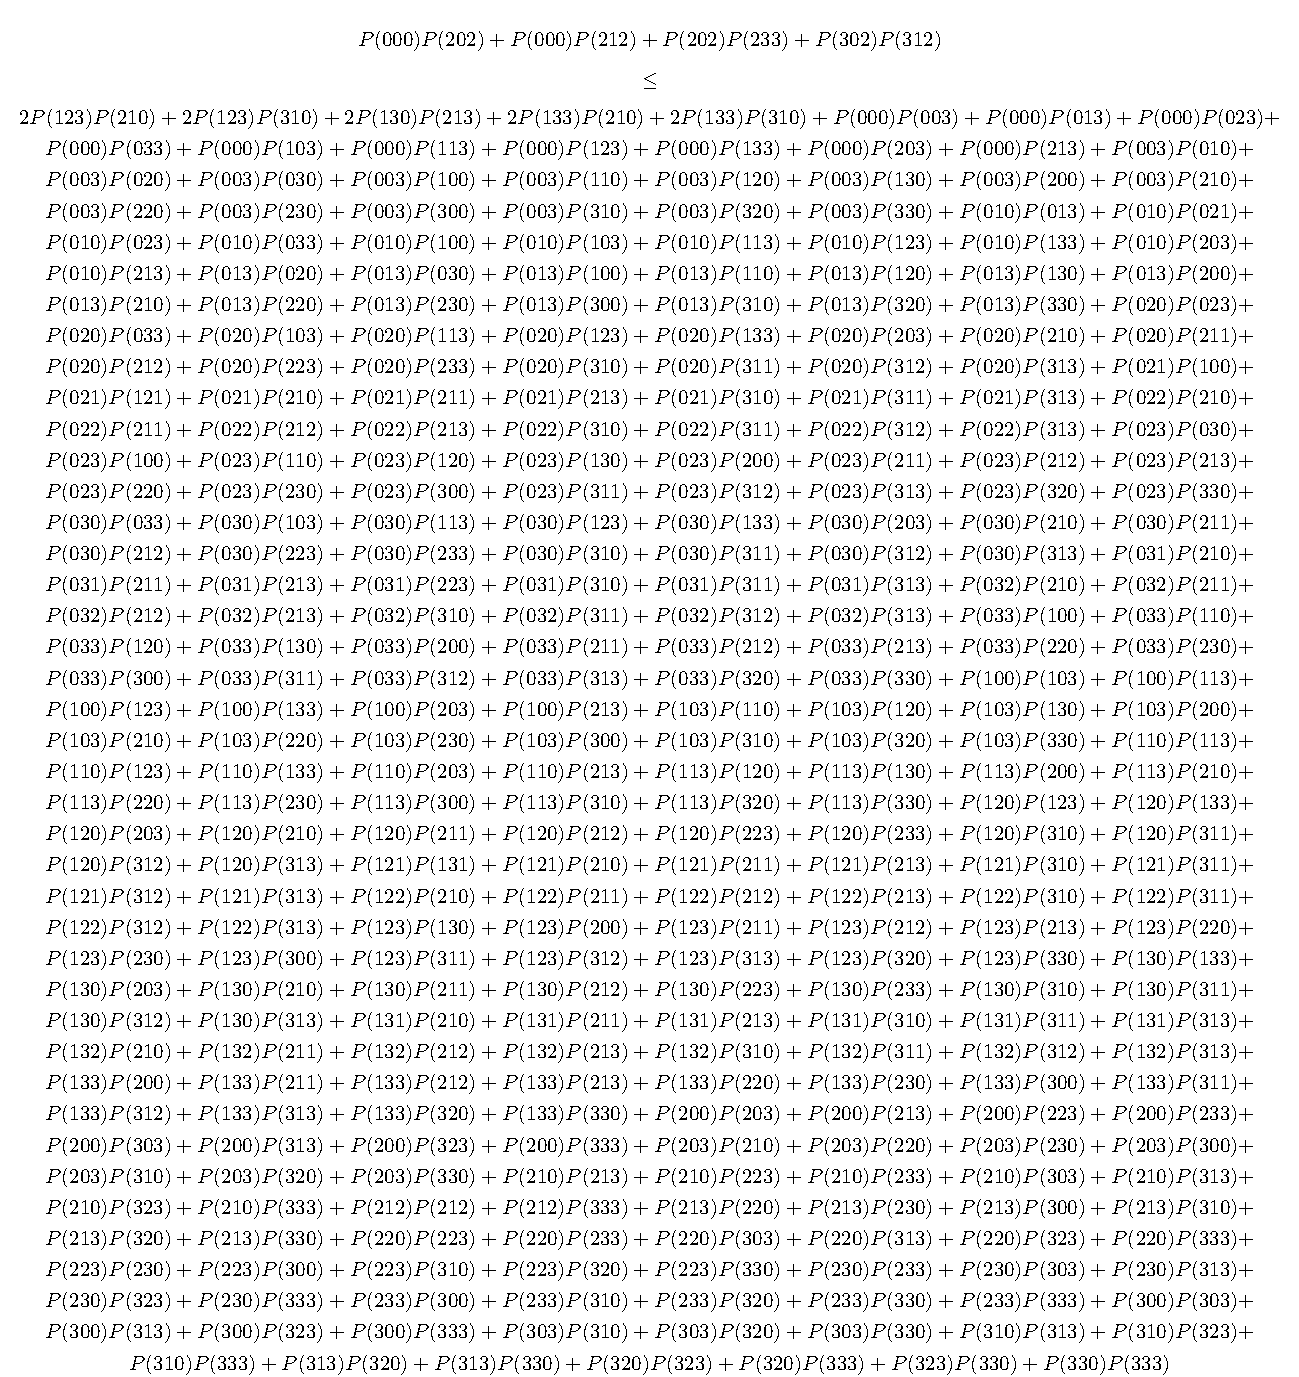
\includegraphics[width=\linewidth]{../../figures/inequalities/no_symwitness_ineq_print_standalone}
    \end{center}
    Note: $\prob\br{abc}$ is shorthand for $\prob[ABC]\br{abc}$.
    \clearpage
    \subsection{Symmetric Web Inflation Inequality}
    \label{sec:symmetic_web_inequality}
    The following is a symmetric causal compatibility inequality for the triangle scenario that is violated by the Fritz distribution outlined in \cref{sec:fritz_distribution} and was derived using the Web inflation of \cref{fig:the_web_inflation}.
    \begin{center}
        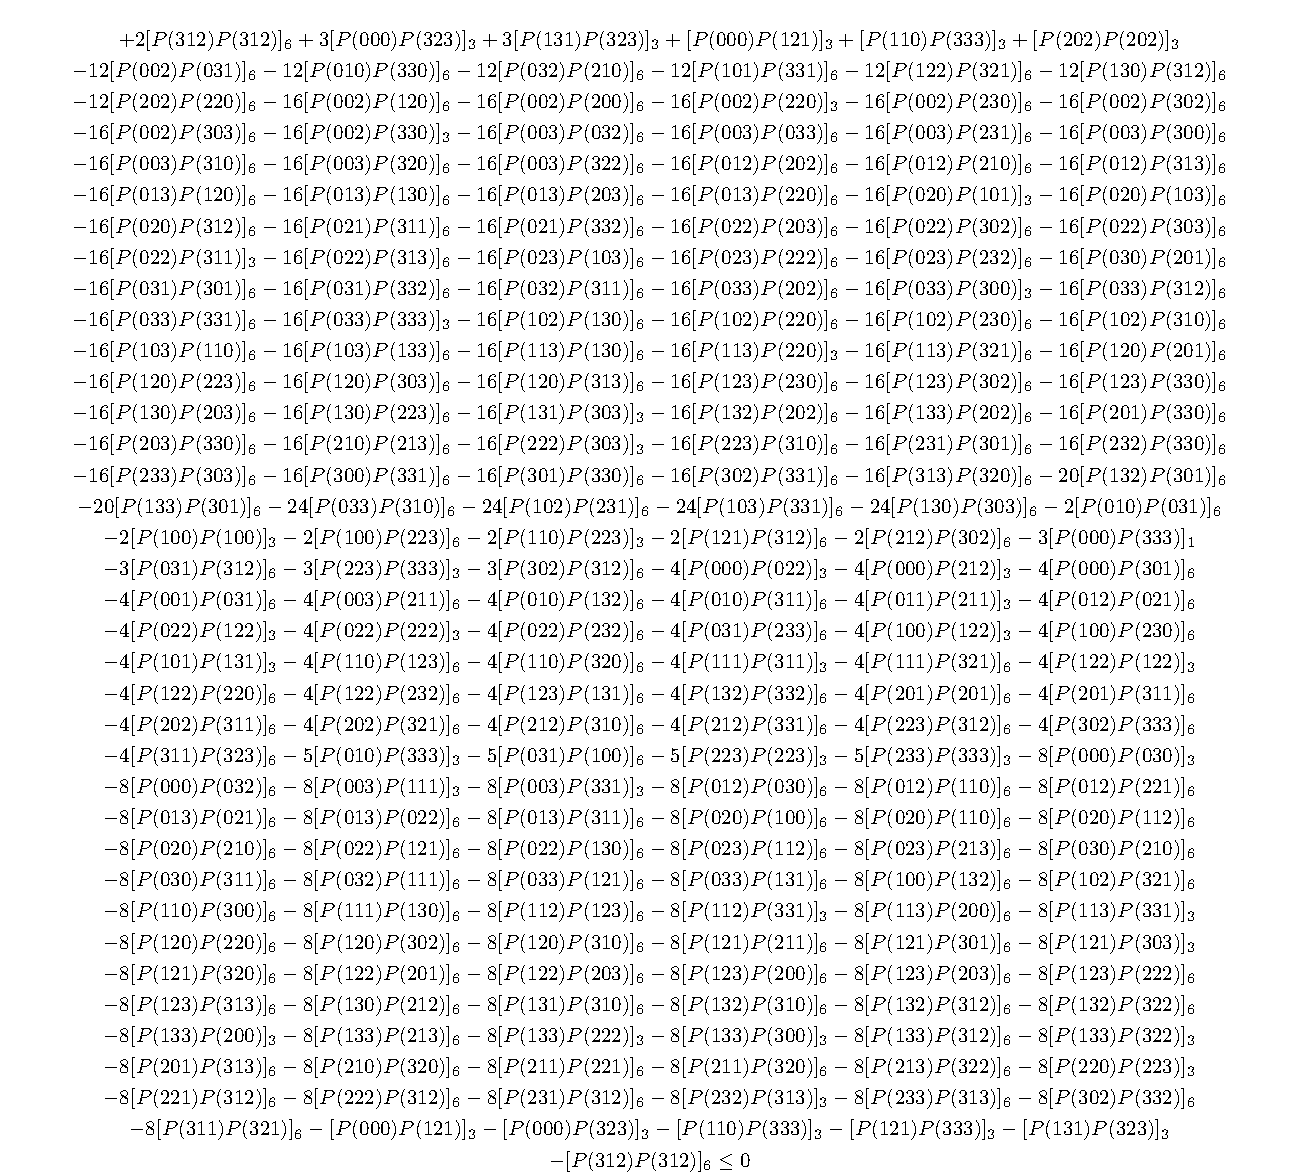
\includegraphics[width=\linewidth]{../../figures/inequalities/MosekCertFritzSym_ineq_standalone}
    \end{center}
    Note: $\prob\br{abc}$ is shorthand for $\prob[ABC]\br{abc}$ and $\bs{P(113)P(330)}_3$ is shorthand for the sum over permutations:
    \[ \bs{P(113)P(330)}_3 = P(113)P(330) + P(131)P(303) + P(311)P(033) \]

\end{document}